\documentclass{beamer}
%\mode<presentation>{\usetheme{Singapore}}
\mode<presentation>{\usetheme{Marburg}}
\usepackage{graphicx}
\usepackage[tikz]{bclogo}
\usepackage{mathtools}
\usepackage{media9}
\presetkeys{bclogo}{
	ombre=true,
	epBord=3,
	couleur = blue!15!white,
	couleurBord = red,
	arrondi = 0.2,
	logo=\bctrombone
}{}
\usepackage{etoolbox}
\makeatletter
\patchcmd{\insertverticalnavigation}%
{\ifx\beamer@nav@css\beamer@hidetext{\usebeamertemplate{section in sidebar}}\else{\usebeamertemplate{section in sidebar shaded}}\fi}%
{{\usebeamertemplate{section in sidebar}}}{}{}
\makeatother
\title{Machine Learning in Astronomy}
\author{Reza Monadi}
\institute{UC Riverside}
\date{May 14, 2020}
\begin{document}
	
	\frame{\titlepage}
	
%	\begin{frame}
%	\centering
%	
\includegraphics[width=\linewidth]{ml.jpg}
%	\tiny{credit: 365datascience.com}
%	
%\end{frame}

	
\section{Overview}
\frame{
	\begin{itemize}
		\uncover<1->{\item Astronomy in \textbf{Big Data} era}
		\uncover<2->{\item Usage of Supervised \textbf{ML} in astronomy}
		\uncover<3->{\item Implementation of unsupervised \textbf{ML} in astronomy }
		\uncover<4->{\item Limitations of \textbf{ML} in astronomy}
	\end{itemize}
	}

\section{Big Data }
\subsection{Definition of BIG DATA}{
	
	\frame{\frametitle{3Vs in astronomy}
		\centering
		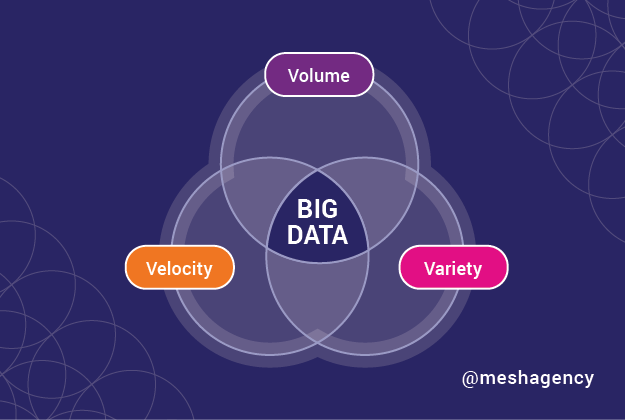
\includegraphics[height=3cm, angle=0,origin=c]{vvv.png}	
		\begin{itemize}
					
			\uncover<1->{\item Volume: larger quantities of data by the advent of better telescopes and surveys }
			\uncover<2->{\item Velocity: Higher speed of incoming  observational data }
			\uncover<3->{\item Variety: multi-wavelength spectroscopic and photometeric data from versatile astronomical objects }
			\end{itemize}
		\centering

}

}
\subsection{Astronomical Surveys}
%\frame{\huge 
%	\centering
%}
%\frame{
%	\frametitle{Sloan Digital Sky Server $\Rightarrow$ 40 TB}
%	\centering
%	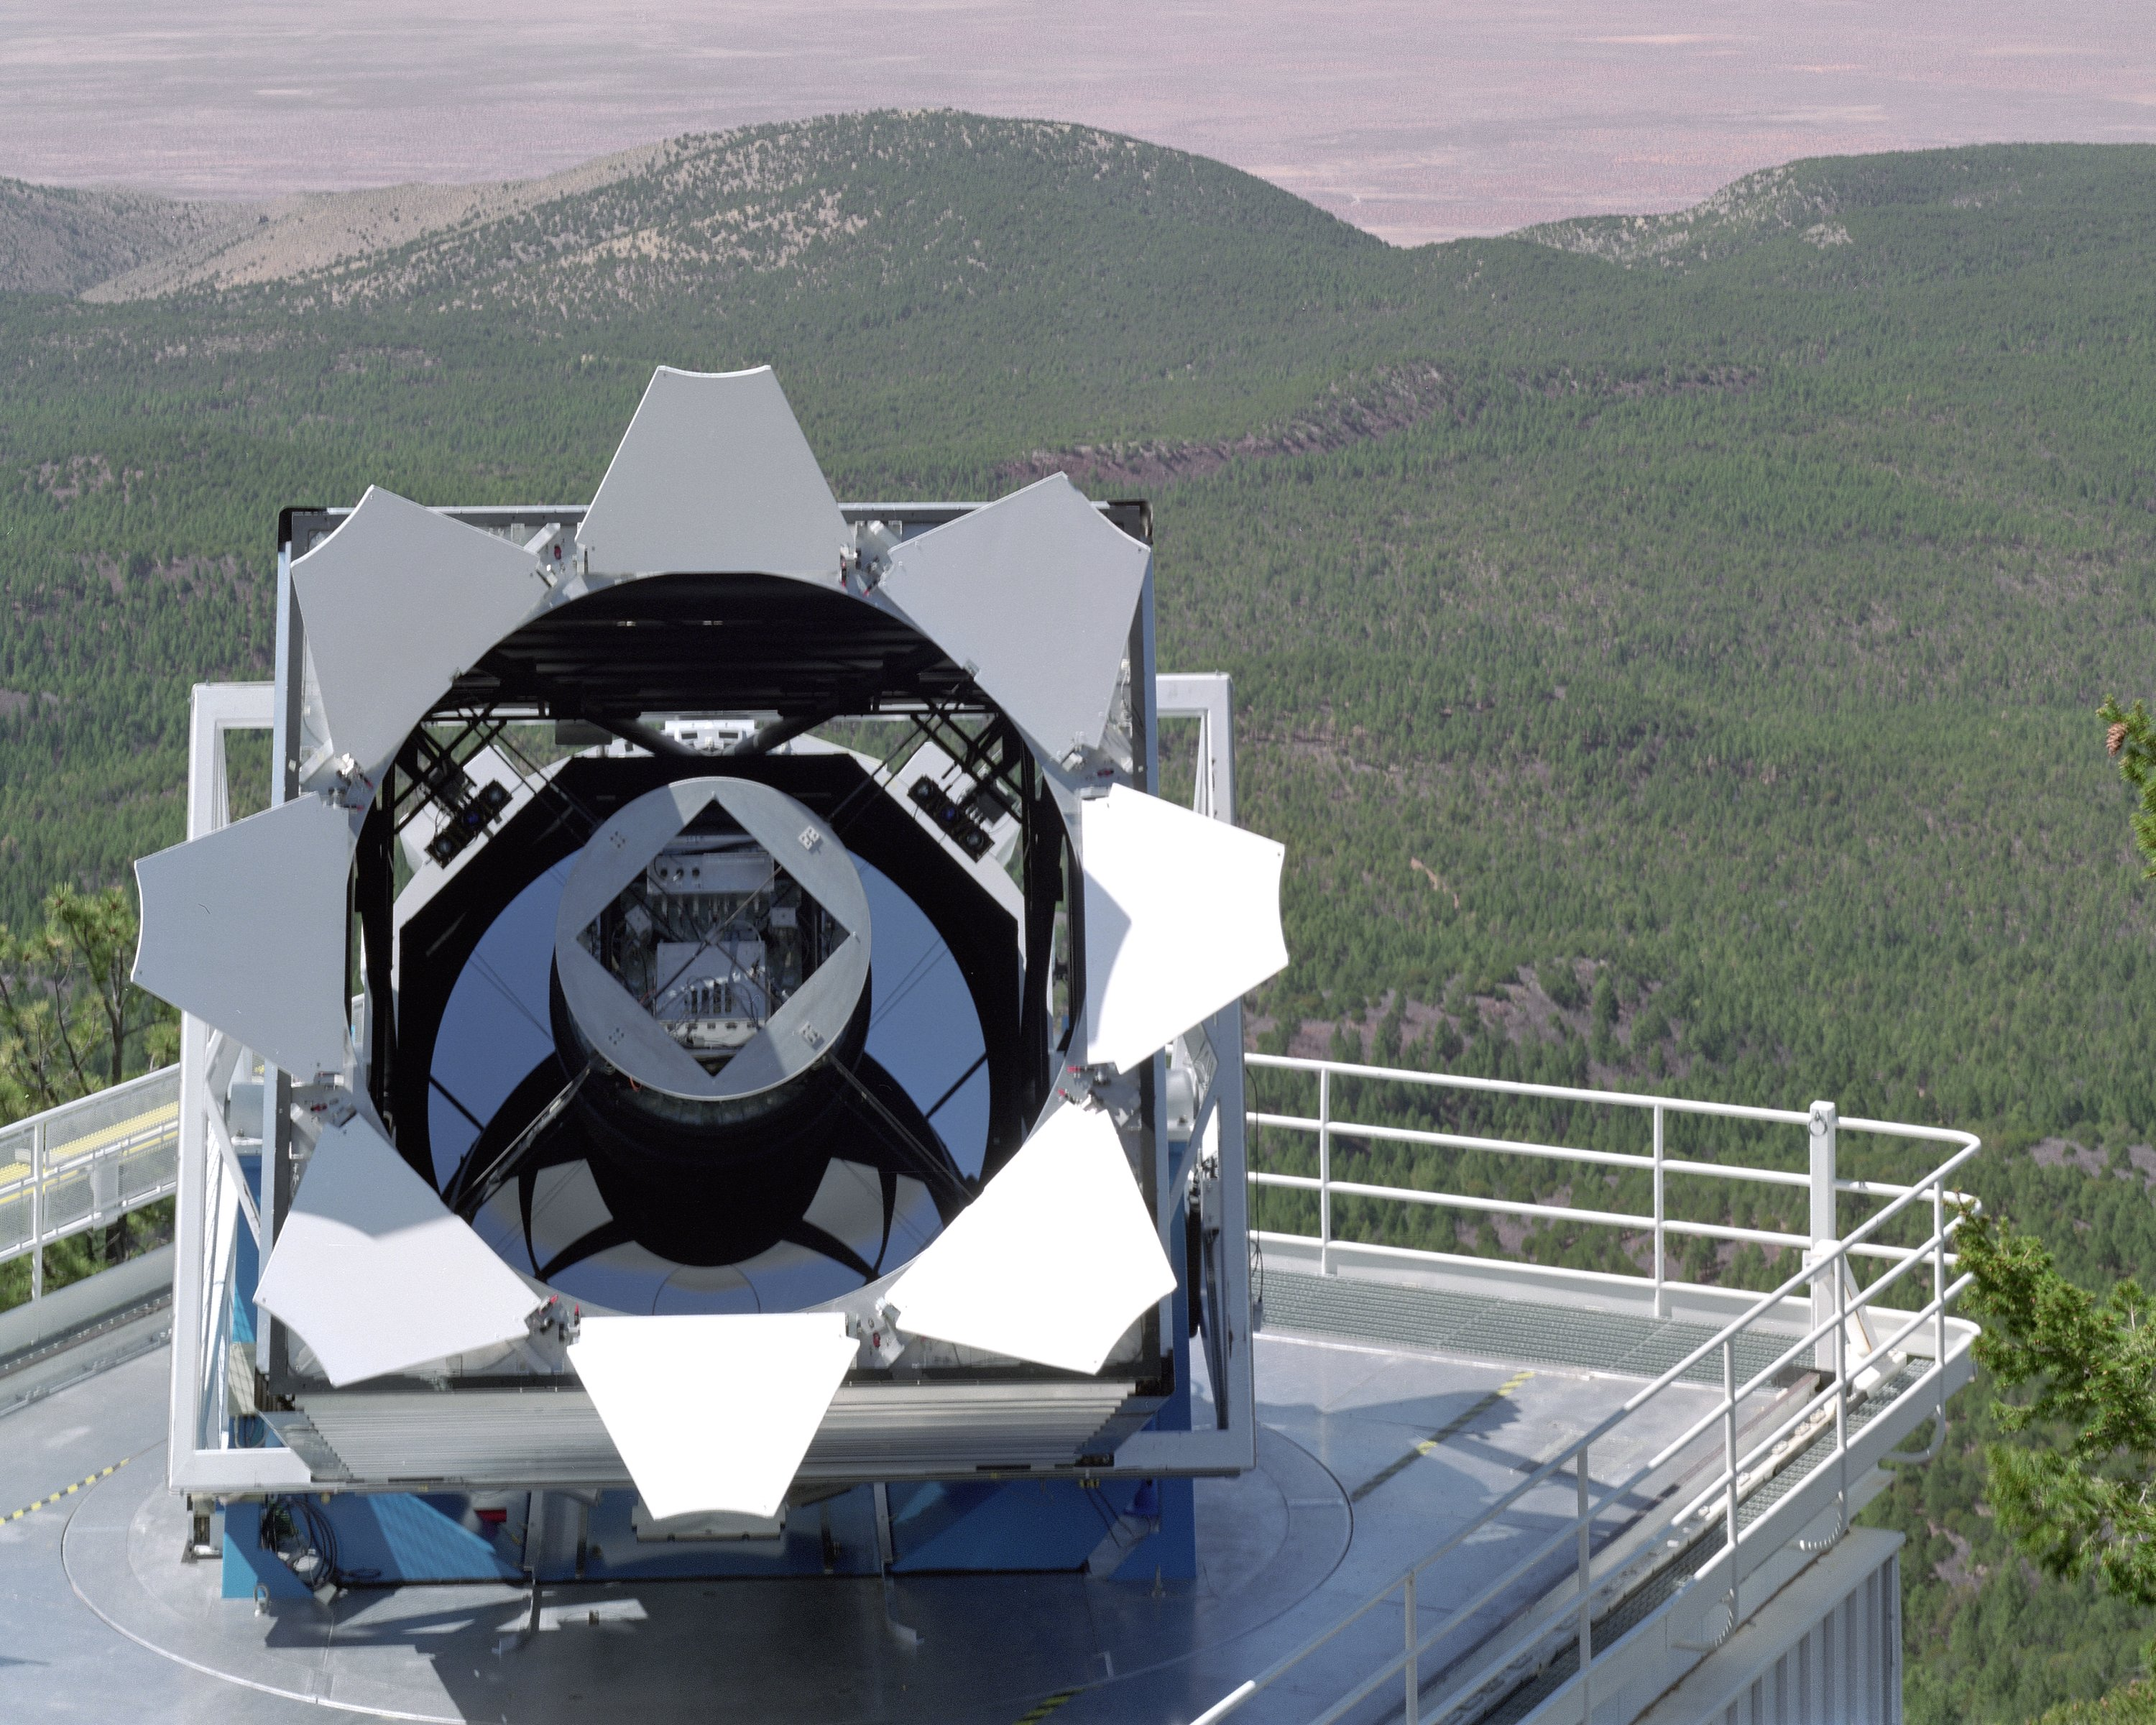
\includegraphics[height=6cm]{sdss-tel}
%}
%\frame{\frametitle{Sloan Digital Sky Server $\Rightarrow$ 40 TB}
%\centering
%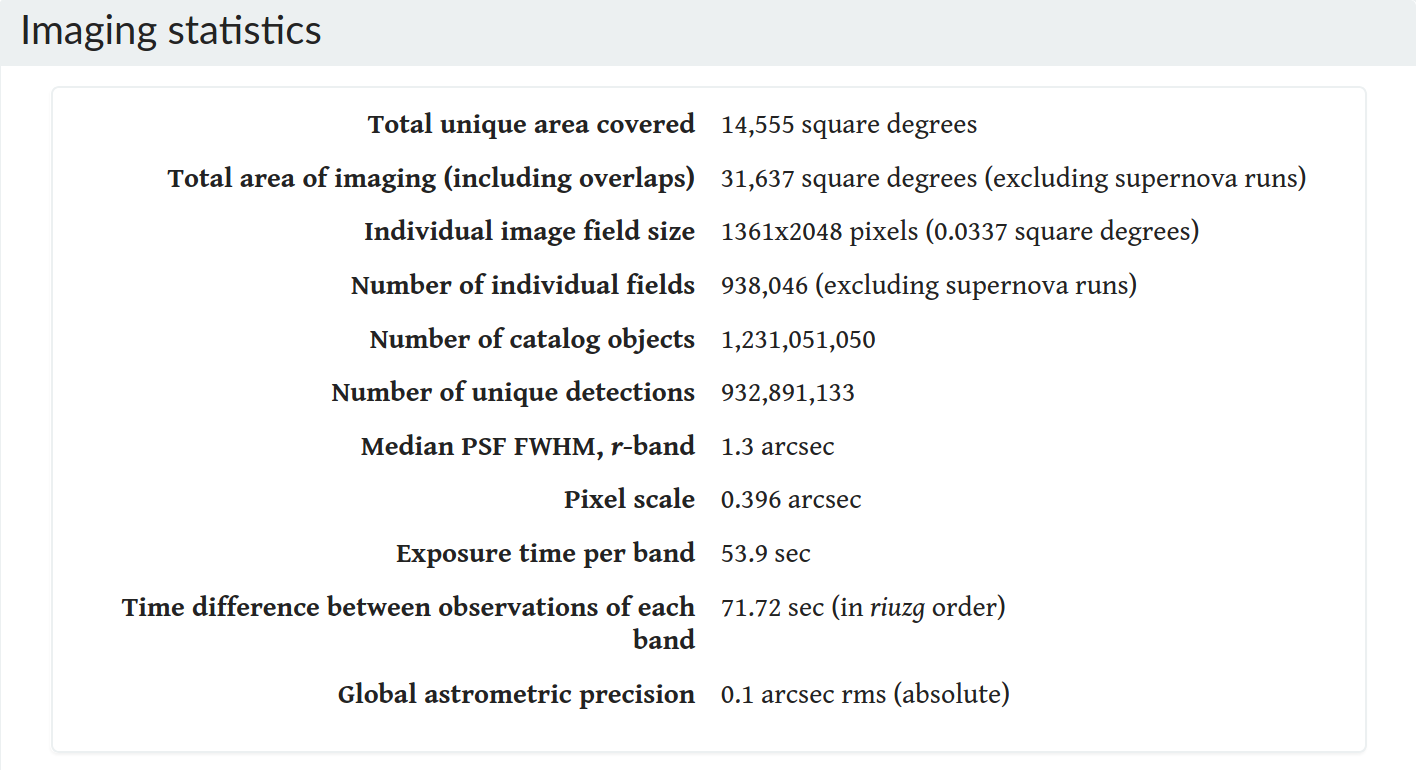
\includegraphics[width=\linewidth]{sdss-imaging-stat}
%
%}
%\frame{\frametitle{Sloan Digital Sky Server $\Rightarrow$ 40 TB}
%	\centering
%	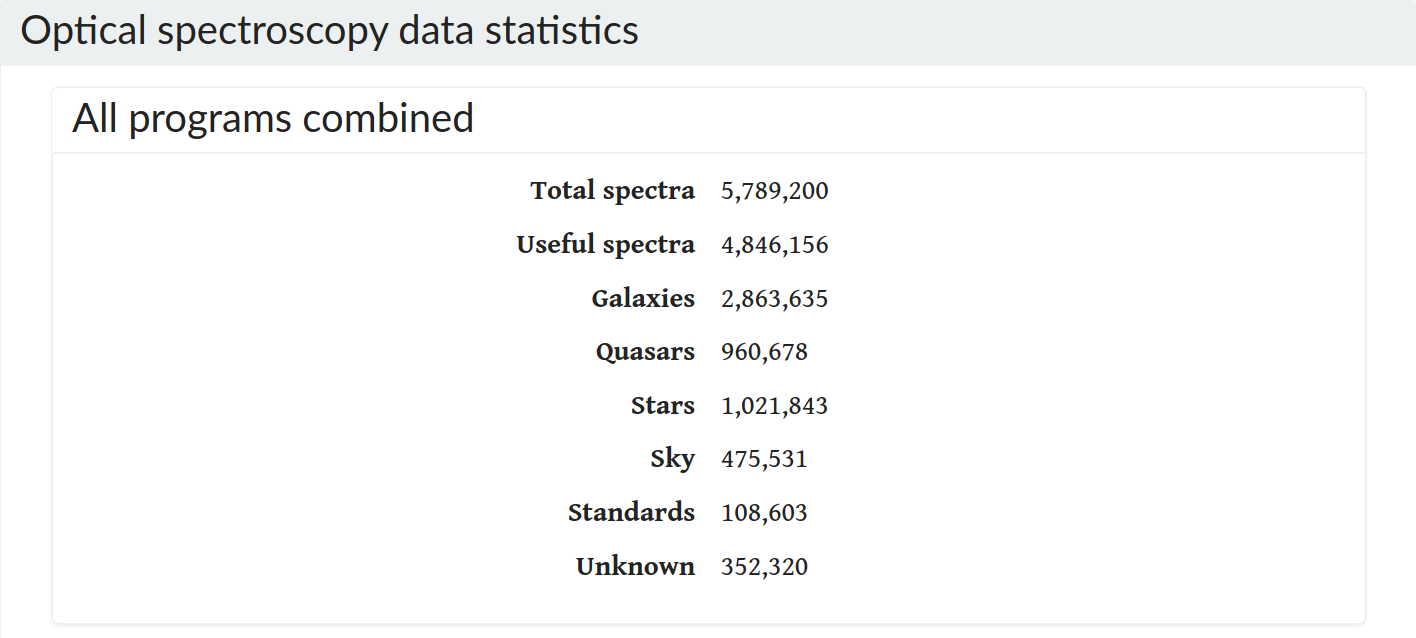
\includegraphics[width=\linewidth]{sdss-spec-stat}
%	
%}
%\frame{\frametitle{Large Synaptic Survey Telescope $\Rightarrow$ 200 PB}
%	\centering
%	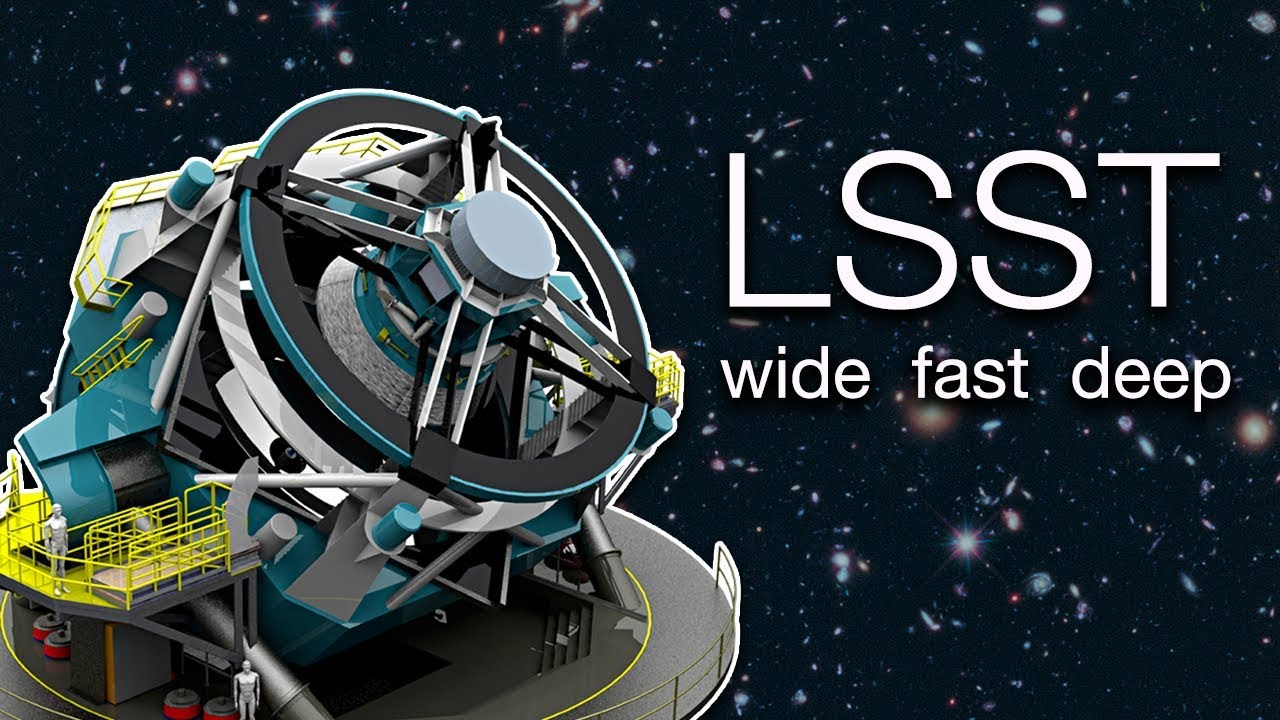
\includegraphics[width=\linewidth]{lsst}}

%\frame{\frametitle{Large Synaptic Survey Telescope $\Rightarrow$ 200 PB}
%\begin{itemize}
%	\uncover<1->{\item 800+ panoramic images each night}
%	\uncover<2->{\item 3.2 billion-pixel camera}
%	\uncover<3->{\item Recording the entire visible sky twice each week}
%	\uncover<4->{\item Each patch of sky will be visited 1000 times}
%\end{itemize}}
%\frame{
%	\frametitle{Zwicky Transient Facility}
%	\centering
%	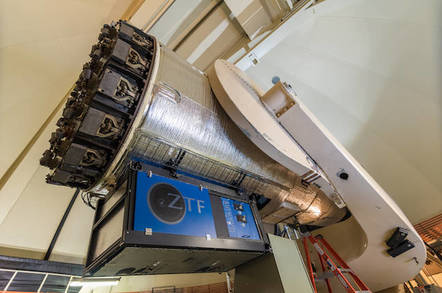
\includegraphics[height=6cm]{ztf_installed}
%}

%\frame{
%	\frametitle{Zwicky Transient Facility}
%	\centering
%	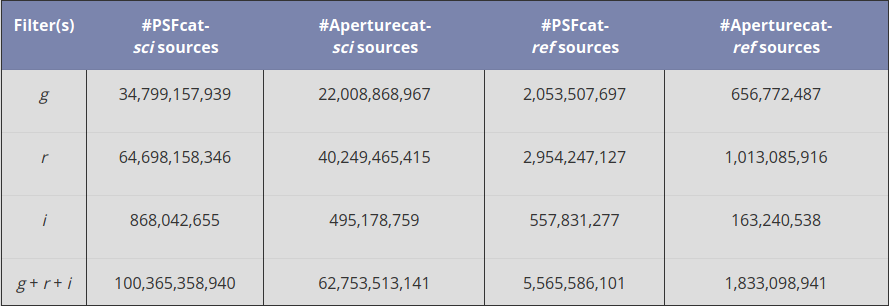
\includegraphics[width=\linewidth]{ztf-stat}
%}

%
%\frame{
%	\frametitle{Dark Energy Spectroscopic Instrument}
%	\centering
%	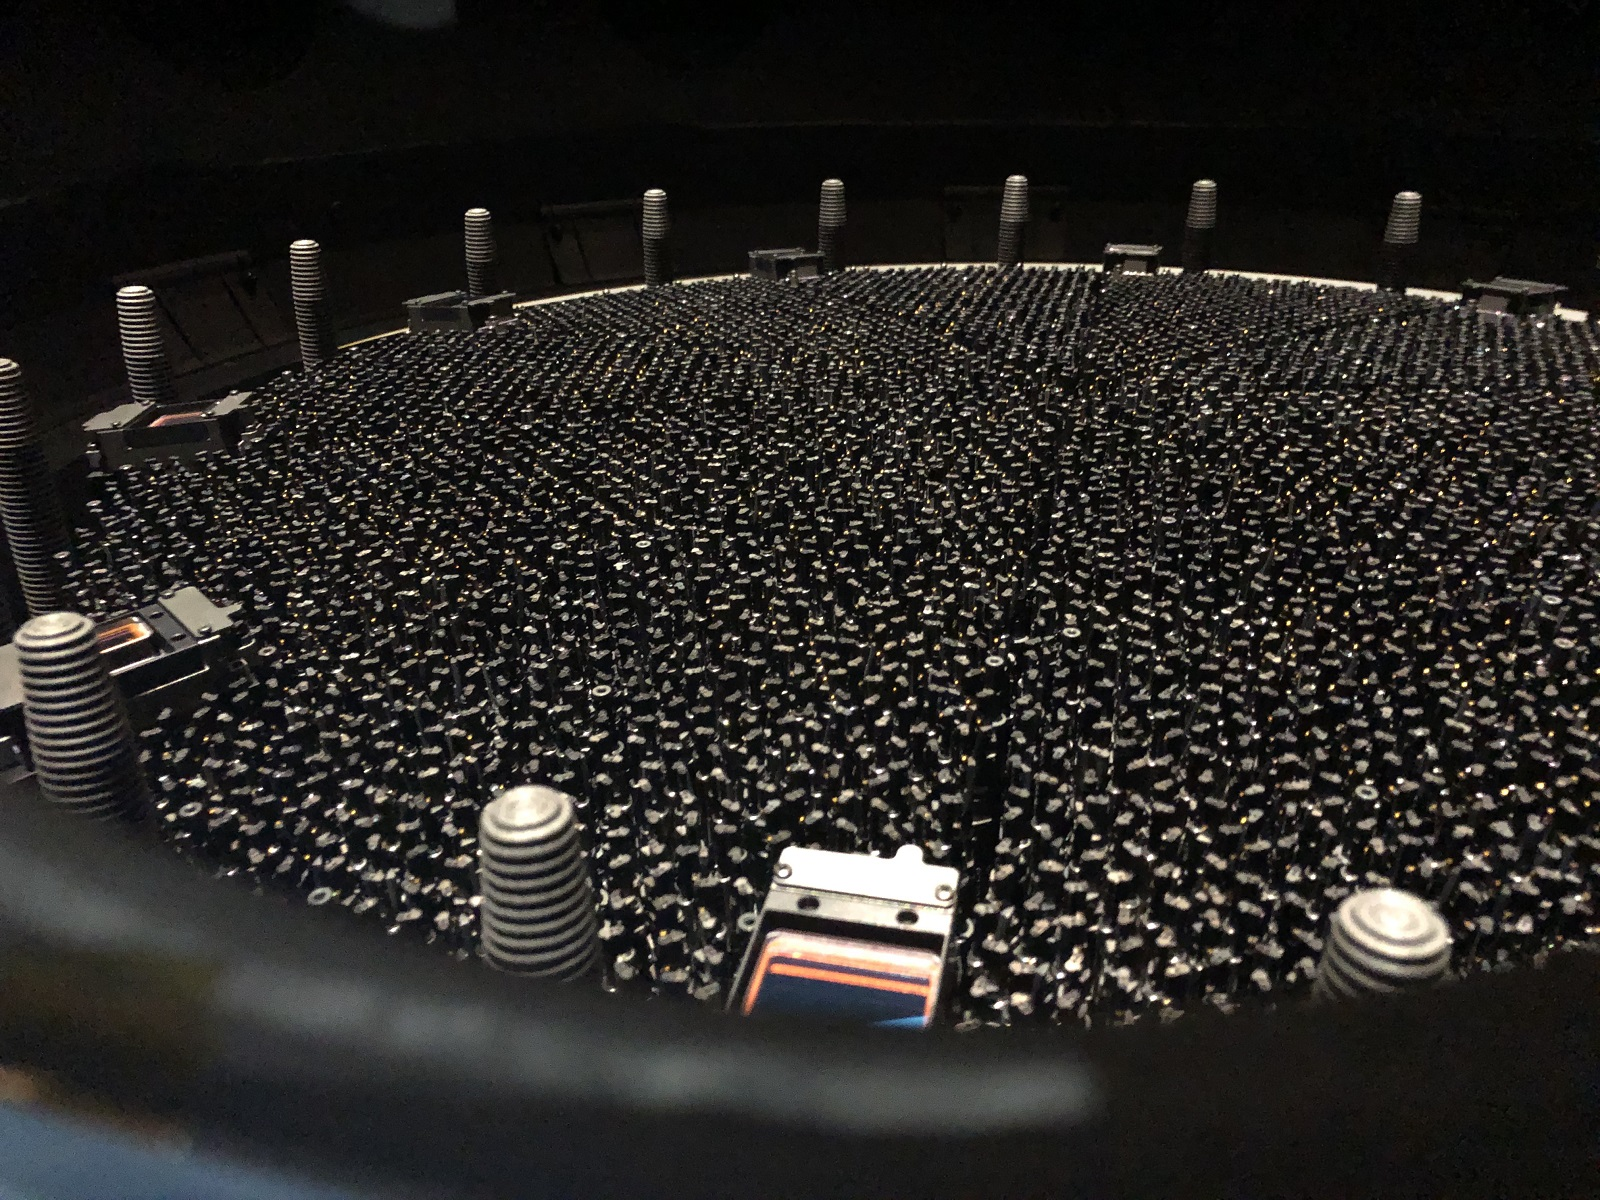
\includegraphics[width=\linewidth]{DESI_2}
%%	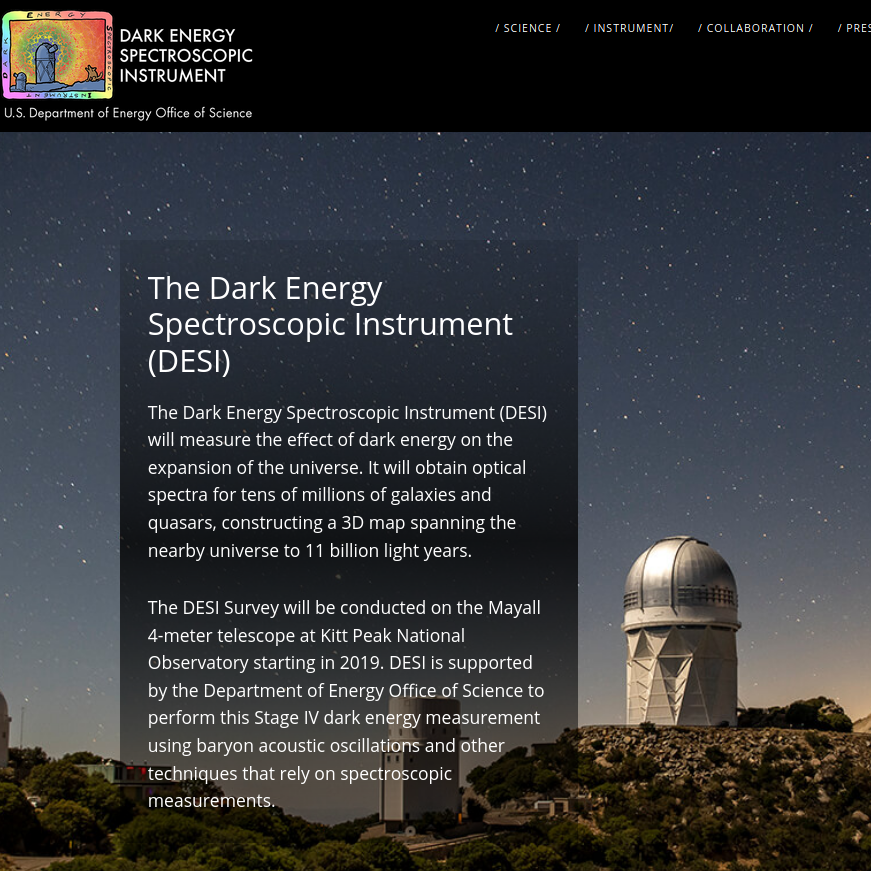
\includegraphics[height=4.55cm]{Desi}
%}
%\frame{
%	\frametitle{Dark Energy Spectroscopic Instrument}
%	\centering
%	\Large{\begin{itemize}
%\uncover<1->{\item Spectra of 25 M galxies, quasars, stars. }
%\uncover<2->{\item 5000 spectra per exposure }
%		\end{itemize}
%	}
%}


\frame{\frametitle{Astronomical surveys are \textcolor{red}{Astronomicaly} growing} 
	
	{\tiny{
\begin{table}[htbp]
	\begin{tabular}{|l|c|}
		\hline
		Sky Server Prokects & Data Volume \\ \hline
		DPOSS (The Palomar Digital Sky Survey) & 3 TB \\ \hline
		2MASS (The Two Micron All-Sky Survey) & 10 TB \\ \hline
		GBT (Green Bank Telescope) & 20 PB \\ \hline
		GALEX (The Galaxy Evolution Explorer) & 30 TB \\ \hline
		SDSS (The Sloan Digital Sky Survey) & 40 TB \\ \hline
		SkyMapper Southern Sky Survey & 500 TB \\ \hline
		PanSTARRS (The Panoramic Survey Telescope and Rapid Response System) & ~ 40 PB expected \\ \hline
		LSST (The Large Synoptic Survey Telescope) & ~ 200 PB expected \\ \hline
		SKA (The Square Kilometer Array) & ~ 4.6 EB expected \\ \hline
	\end{tabular}
	\label{}
\end{table}}}
%	\centering
	\begin{figure}
\tiny{SKA}
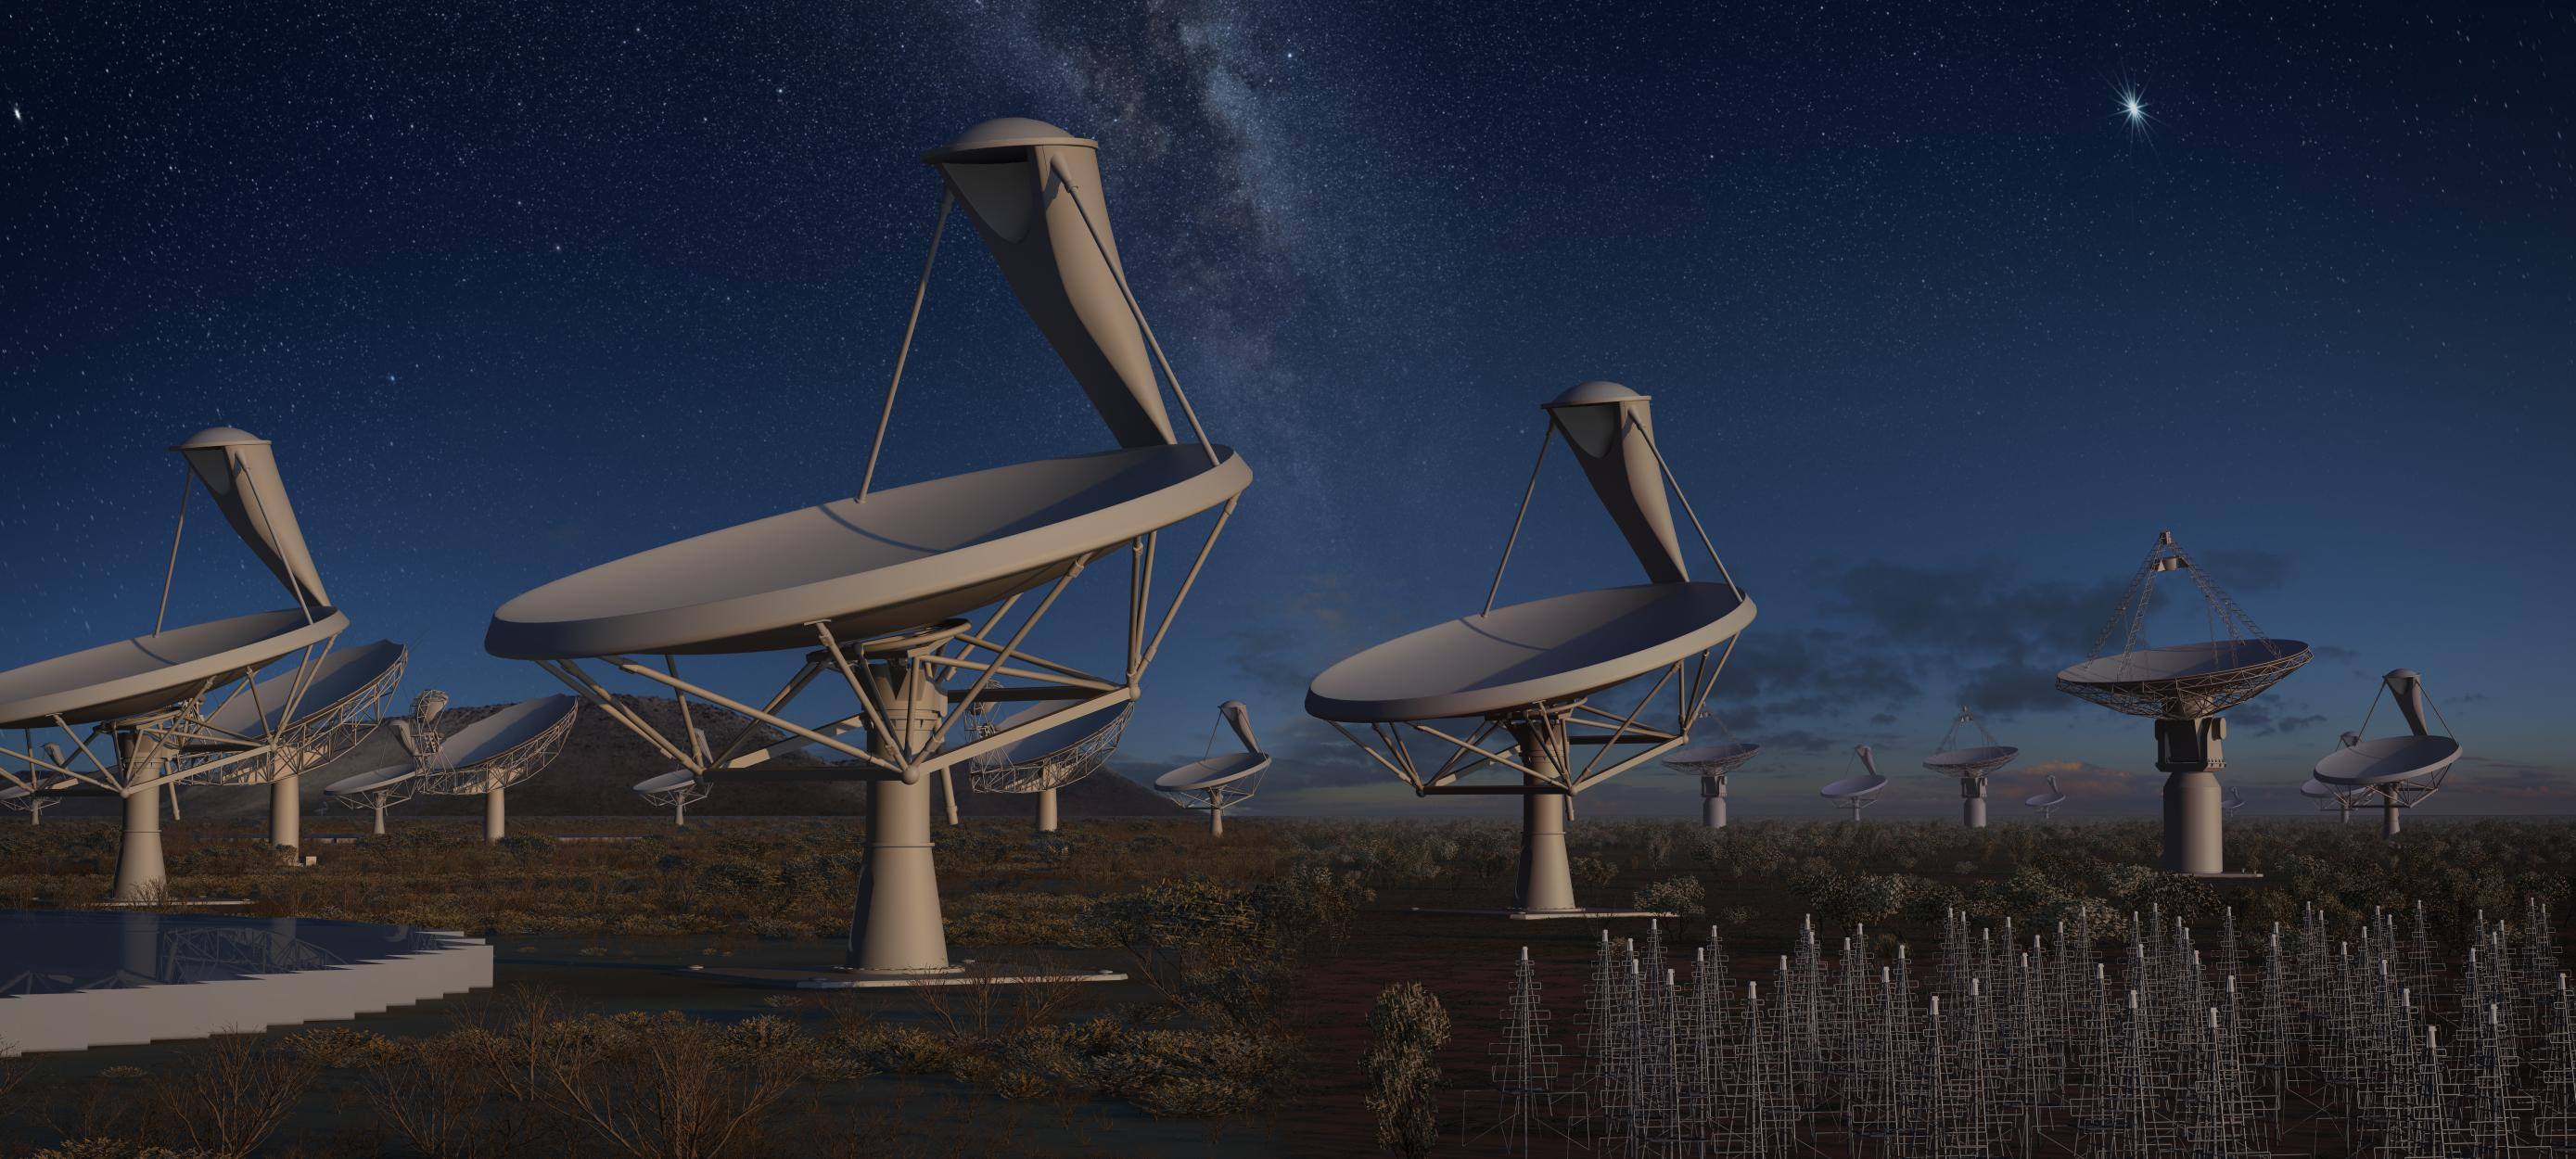
\includegraphics[height=1.5cm, angle=-5]{ska}
	\tiny{DESI}
		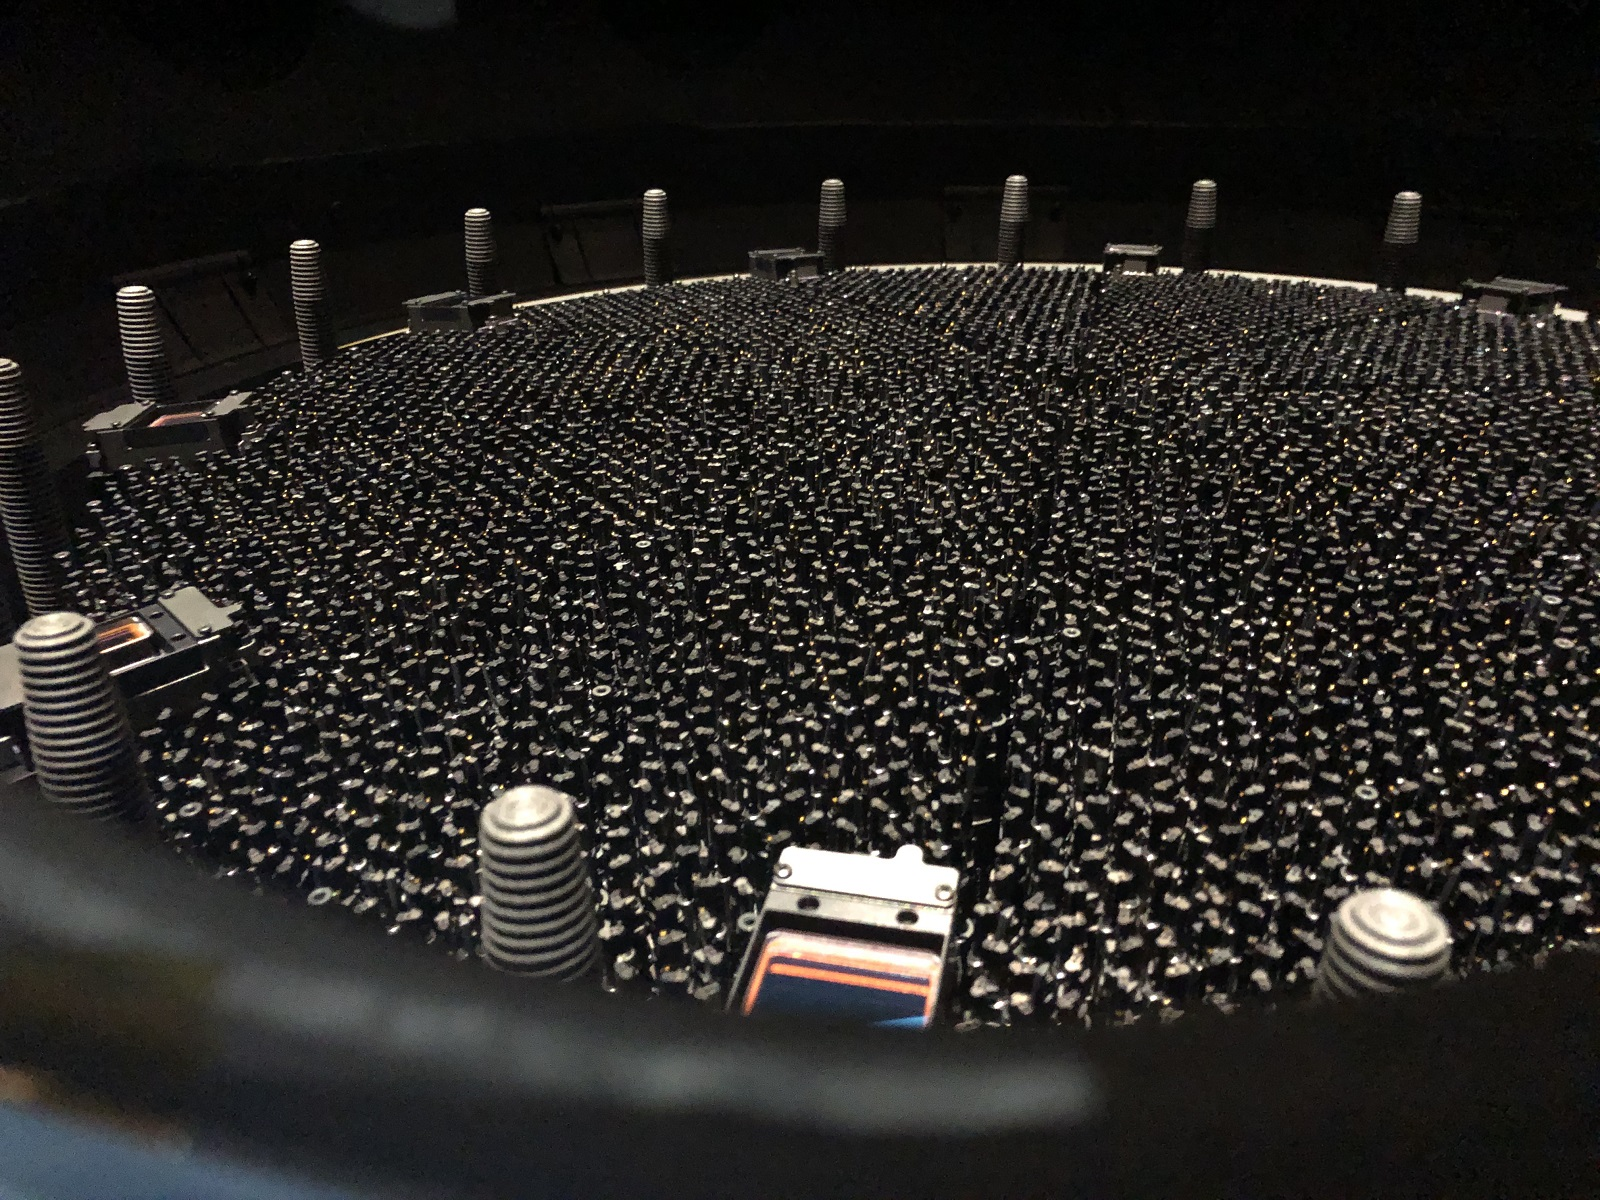
\includegraphics[height=1.5cm, angle=5]{DESI_2}
	\end{figure}
\begin{figure}
\end{figure}
\begin{figure}
	\tiny{ZFT}
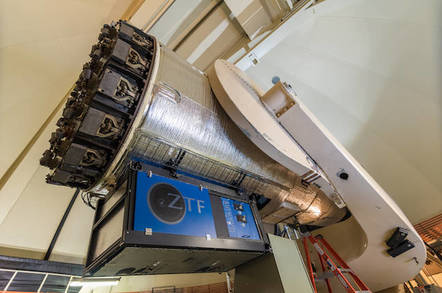
\includegraphics[width=2cm, angle=5]{ztf_installed}
\tiny{LSST}
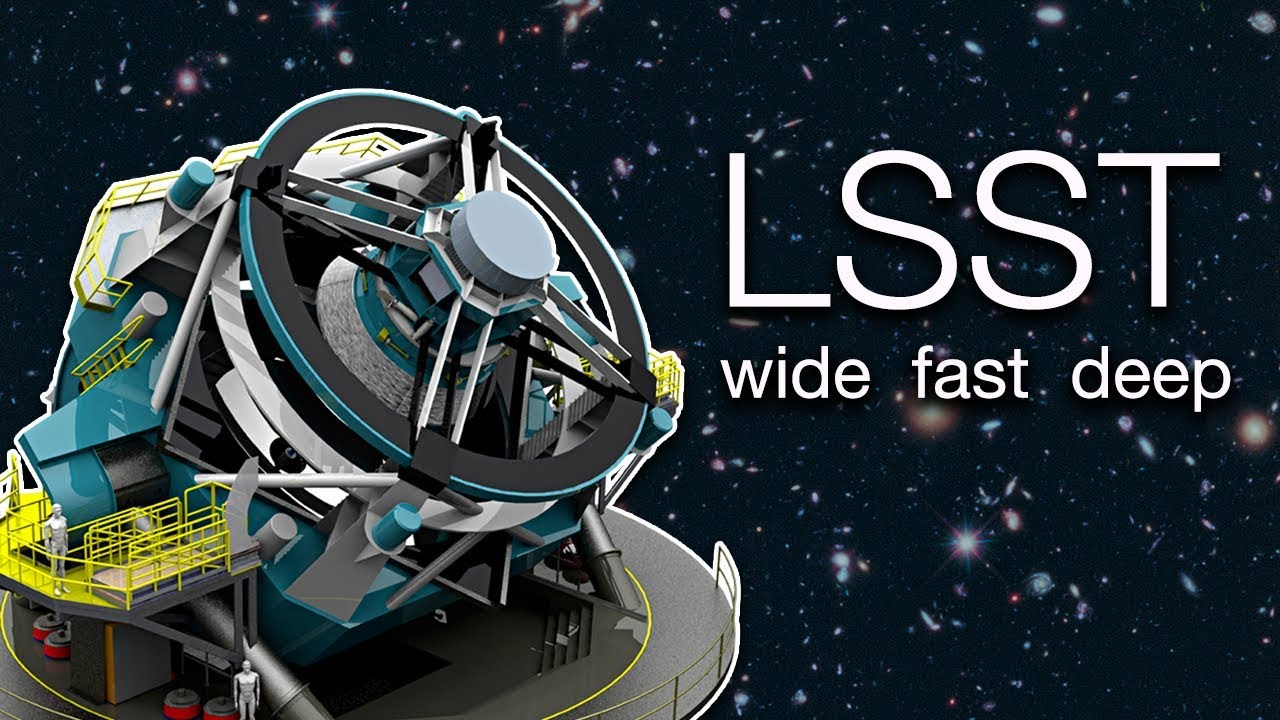
\includegraphics[width=2cm, angle=-5]{lsst}
\end{figure}
%\tiny{
%	\begin{block}
%		\uncover<1->{Large surveys}
%		\uncover<2->{$\Rightarrow$}
%		\uncover<3->{Big Data}
%		\uncover<4->{$\xRightarrow{ML}$ \\ }
%		\uncover<5->{\centering Astronomy Knowledge}
%		
%\end{block} }
}


%
%
%
%}

%\frame{\frametitle{BIG DATA and ML}
%	
%	%	\begin{columns}[c]
%	%		\column{.5\textwidth}
%	%		\begin{center}
%	%			\includegraphics[scale=0.3]{}
%	%		\end{center}
%	%		\column{.5\texwidth}
%	%		\begin{center}
%	%			\includegraphics[scale=0.3]{} 
%	%		\end{center}
%	%	\end{columns}
%	
%	
%	
\includegraphics[width=0.5\linewidth]{old-wise.jpeg}
%		
\includegraphics[width=0.45\linewidth]{clumsy.jpeg}
% }


\section{Supervised ML}{
%\frame{\frametitle{How Supervised ML works}
%\begin{figure}
%	
%%	\caption{}
%%	\label{fig:example-supervised}
%\end{figure}
%}
%
%}
\subsection{Overview}
\frame{\frametitle{Stages of Supervised Learning}
	\centering
	\begin{figure}
		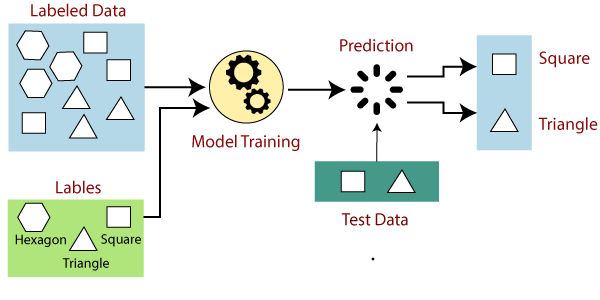
\includegraphics[width=4cm]{example-supervised.png}
		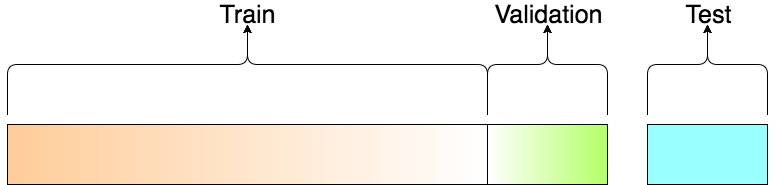
\includegraphics[width=4cm]{tvt.png}
	\end{figure}
	
	
	\begin{itemize}
		\uncover<1->{\item Training: 
			\begin{enumerate}
				\uncover<2->{\item Select a model }
				\uncover<3->{\item Set up hyper-parameters of model}
				\uncover<4->{\item Teach the machine by training set}
				\uncover<6->{\item Validate the hyper-parameters  }
				\uncover<7->{\item Select the optimum hyper-parameters}
		\end{enumerate} } 
		\uncover<8->{\item Testing: 
			\begin{enumerate}
				\uncover<9->{\item Test learned model by an unseen part of the data-set. }
				\uncover<10->{\item Select the best model and use it for predictions.}
		\end{enumerate} } 
	\end{itemize}
	
}

\subsection{Support Machine Vector }

\frame{ 
	\frametitle{How Support Vector Machine  Works?}
	\centering
	%\includemovie{1cm}{1cm}{svm1.gif}
	\uncover<1->{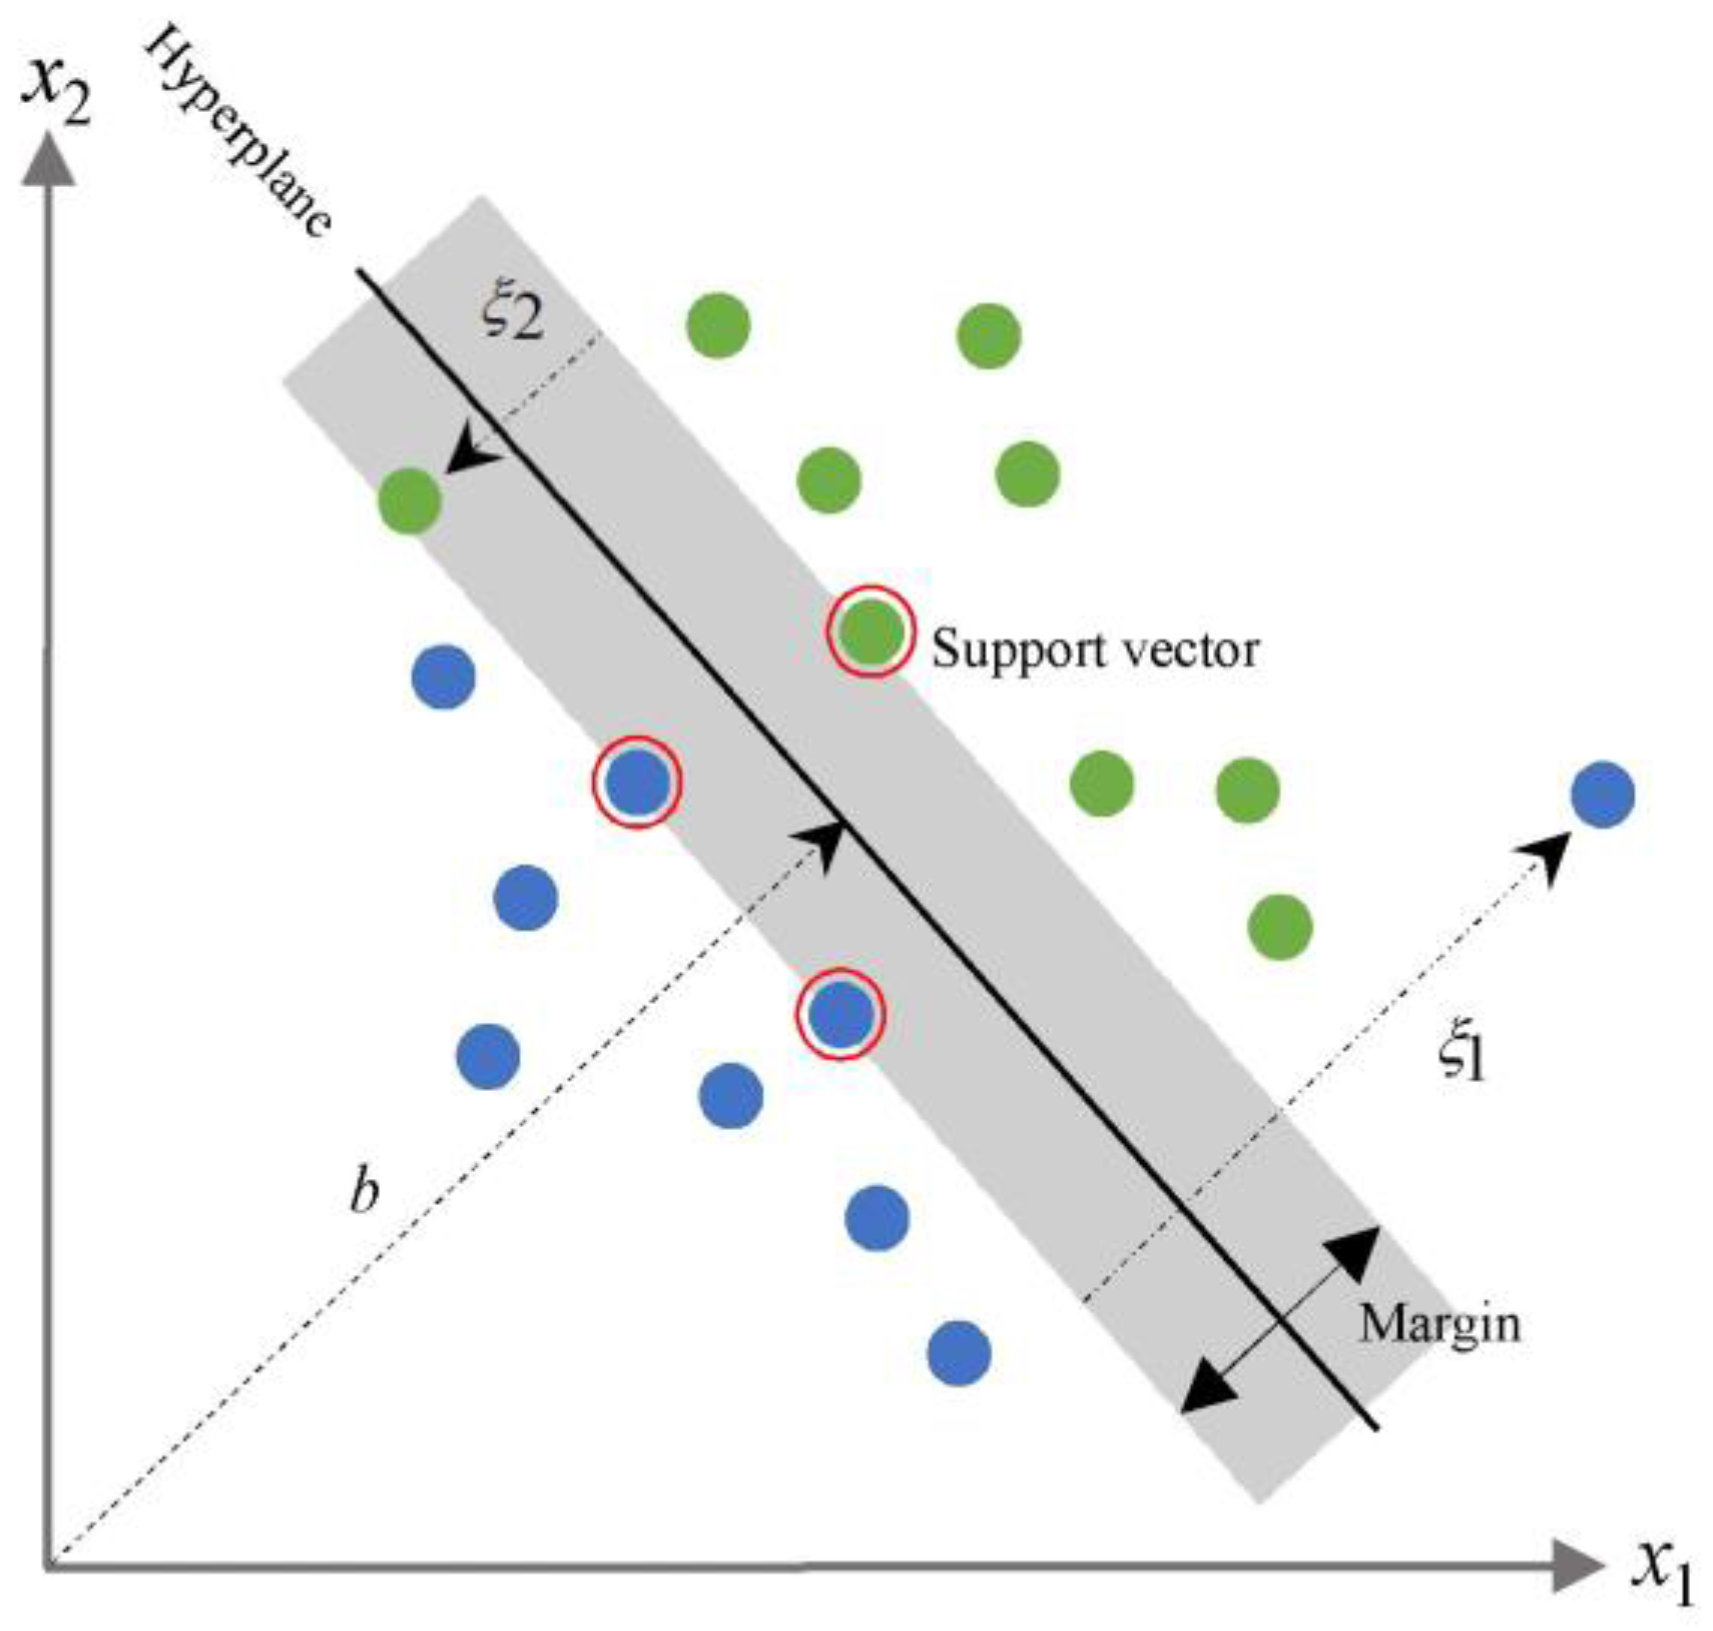
\includegraphics[height=7cm]{svm-2.png}}
%	\uncover<2->{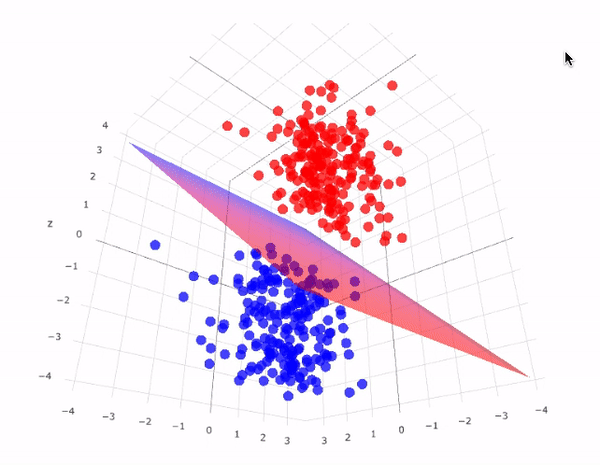
\includegraphics[height=3cm]{svm1-0.png}}
}

%\frame{ 
%	\frametitle{Hyper-plane in Support Vector Machine}
%	\centering
%	%\includemovie{1cm}{1cm}{svm1.gif}
%	
%	
%}
\frame{
	\frametitle{ Classifying Pre-Main-Sequence Stars using SVM }
	
	\centering
	%\includemovie{1cm}{1cm}{svm1.gif}
	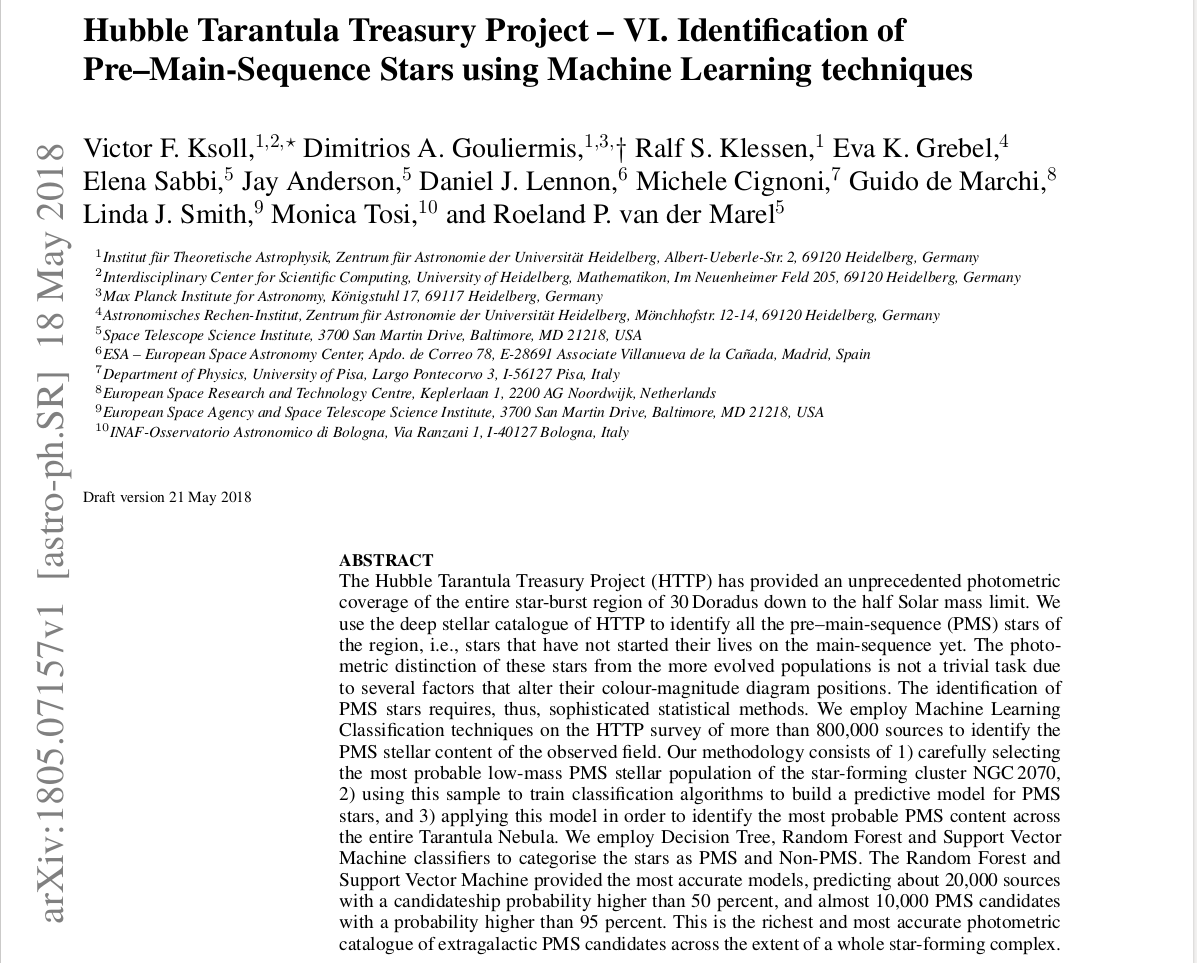
\includegraphics[height=7cm]{svm-paper}}

\frame{
	\frametitle{ Classifying Pre-Main-Sequence Stars using SVM }
	
	\centering
	%\includemovie{1cm}{1cm}{svm1.gif}
	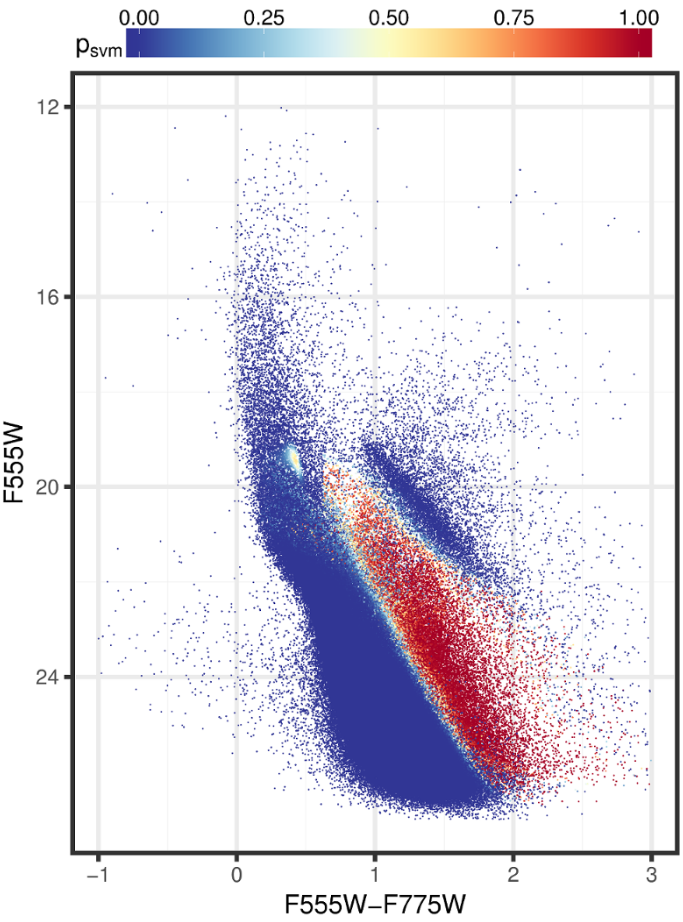
\includegraphics[height=7cm]{svm-example}
} 
\subsection{Decision Tree } 
\frame{\frametitle{How Decision Tree works?}
	\centering
	%\includemovie{1cm}{1cm}{svm1.gif}
	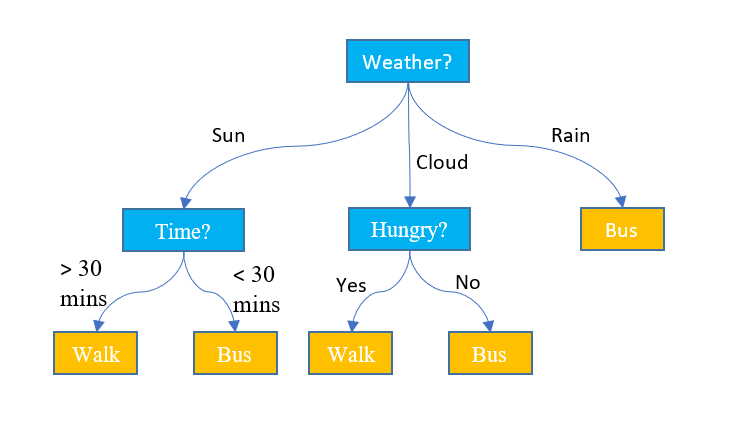
\includegraphics[height=6cm]{DT-works}}


\frame{\frametitle{Using DT for classifying galaxies and stars in SDSS?}
	\centering
	
	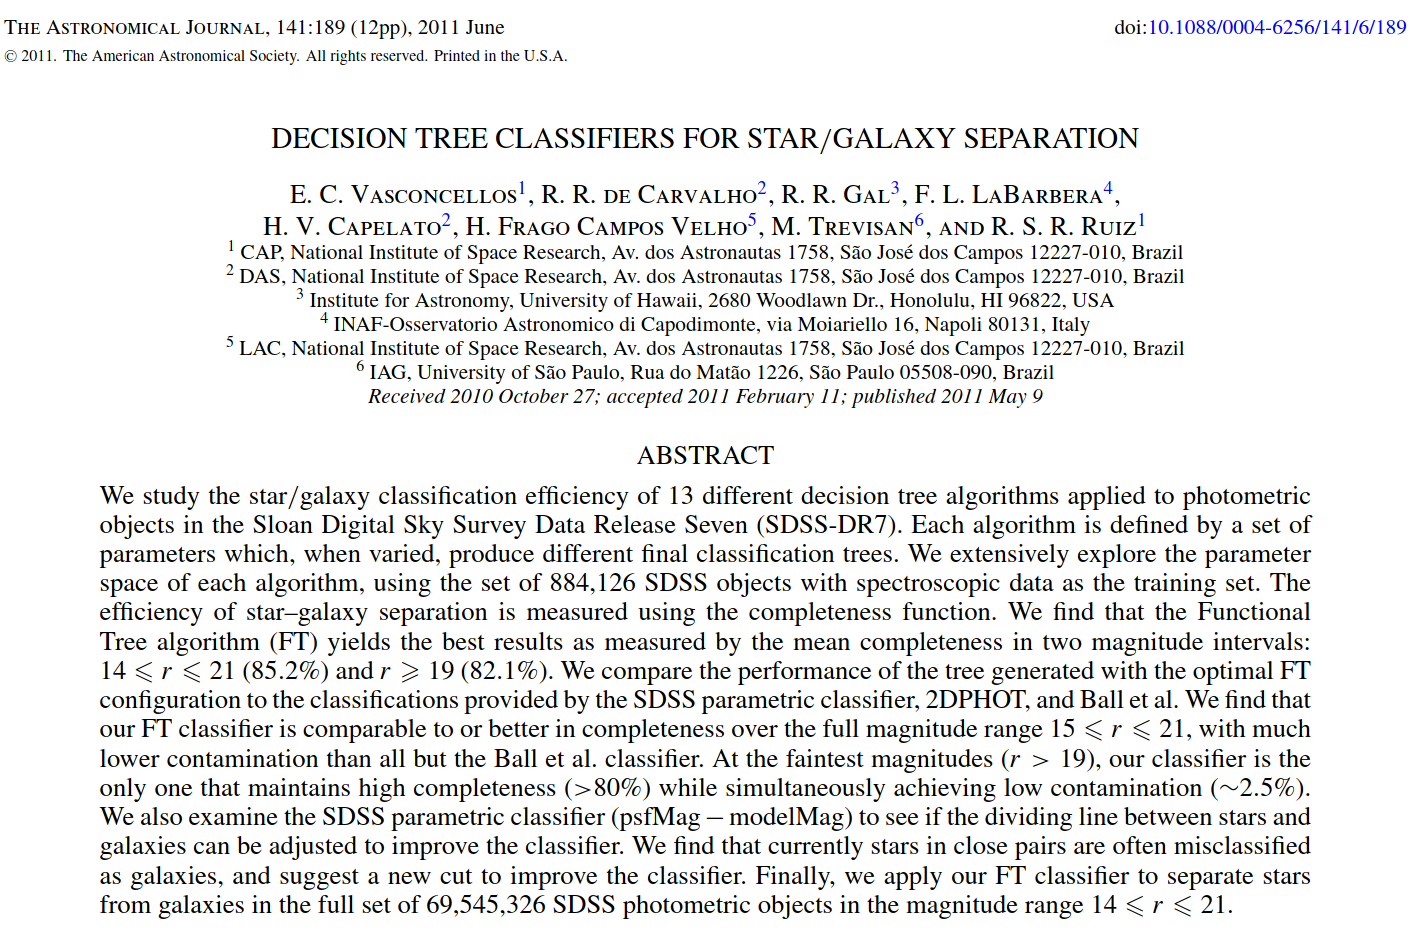
\includegraphics[height=6cm]{DT-paper}
	
}

\frame{\frametitle{Using DT for classifying galaxies and stars in SDSS?}
	\centering
	%\includemovie{1cm}{1cm}{svm1.gif}
	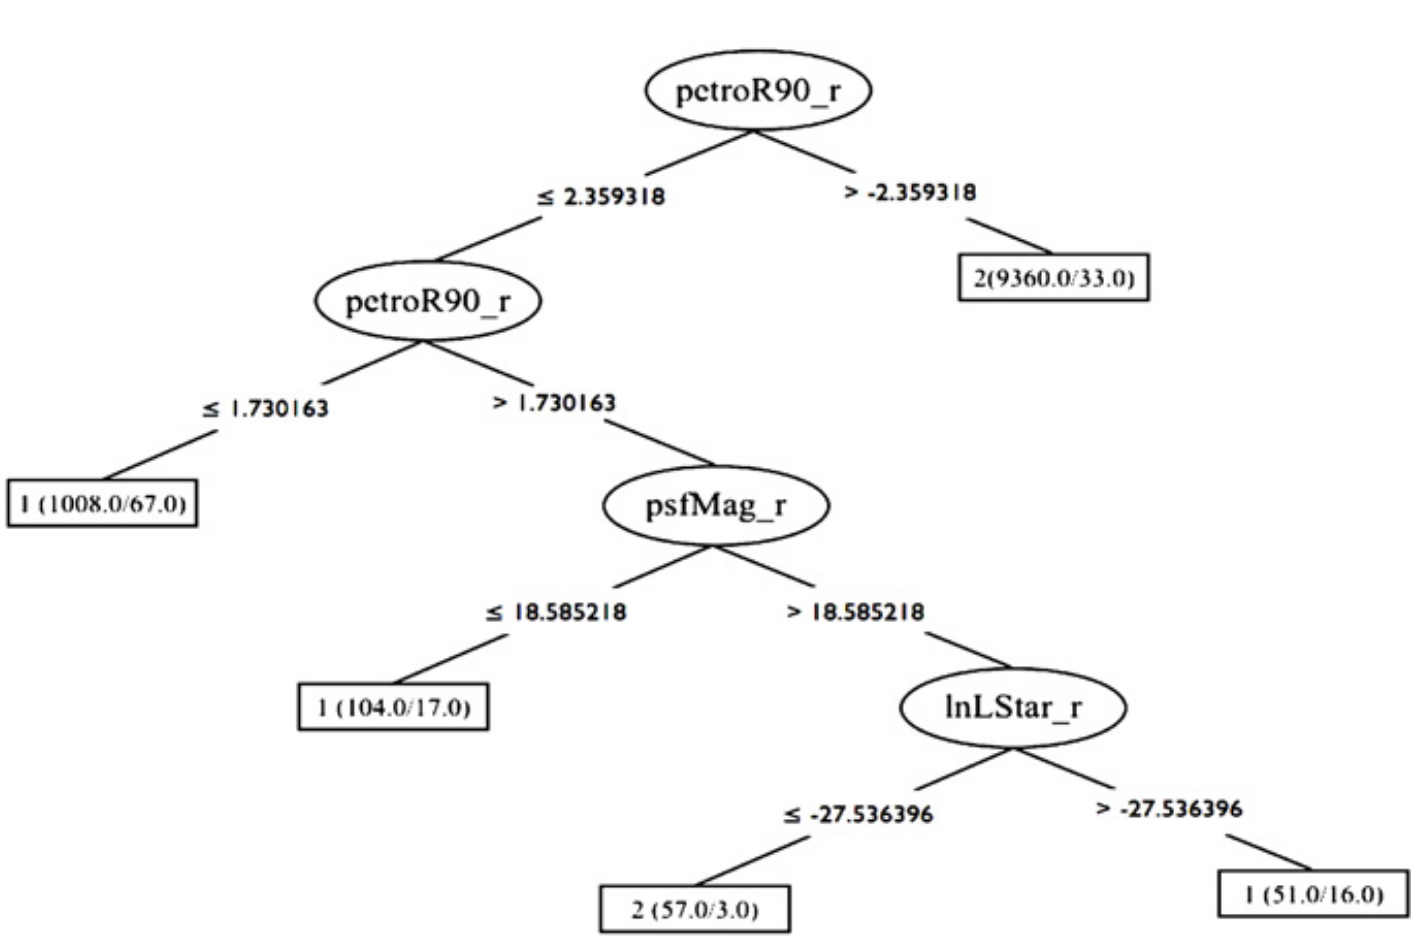
\includegraphics[height=6cm]{DT-example}
	
}

\subsection{Neural Network}
\frame{\frametitle{How Neural Network works?}
	\centering
	%\includemovie{1cm}{1cm}{svm1.gif}	
	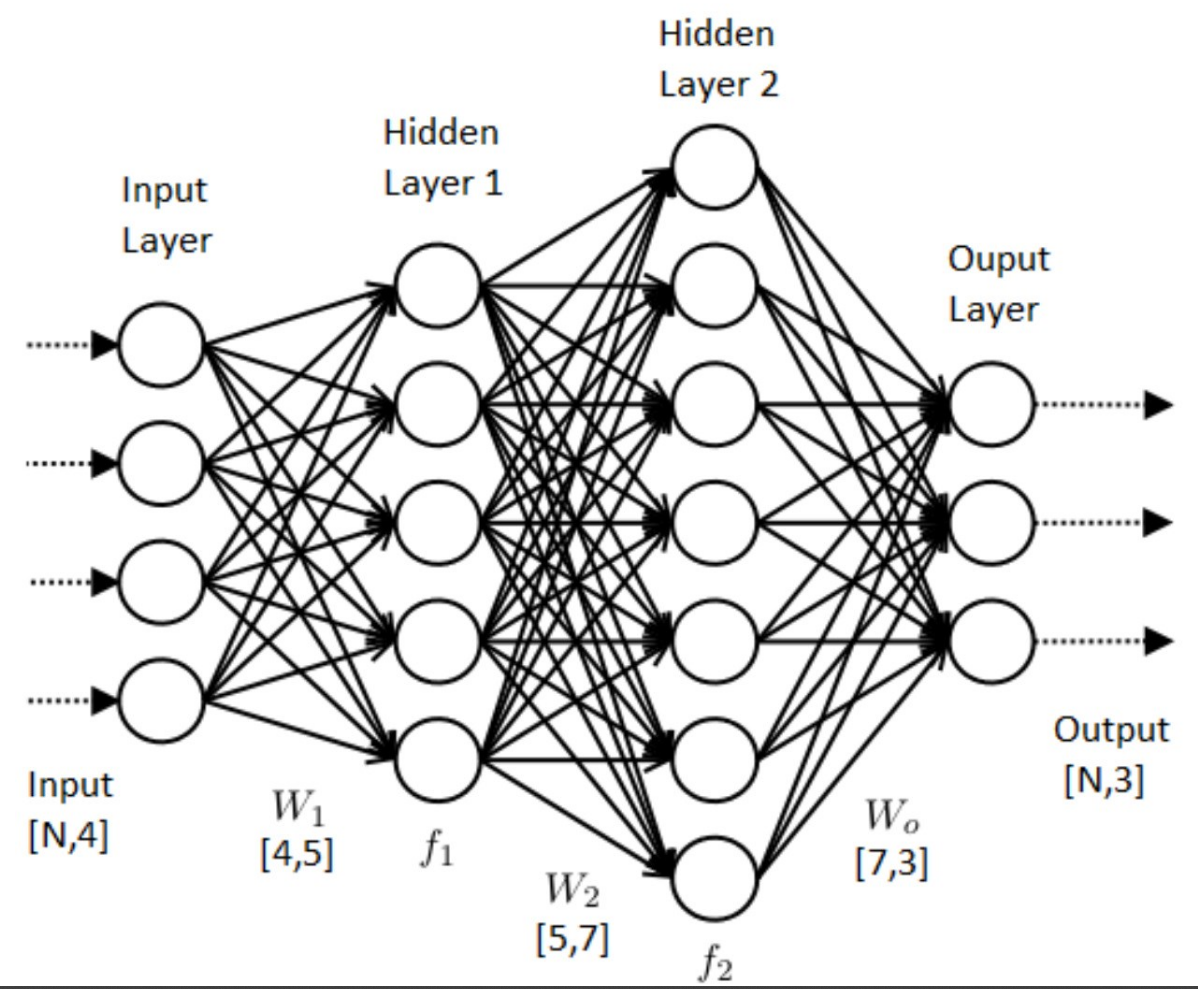
\includegraphics[height=7cm]{NN-works-3}
	
}

\frame{\frametitle{Convolutional Neural Network and DLAs}
	\centering
	%\includemovie{1cm}{1cm}{svm1.gif}	
	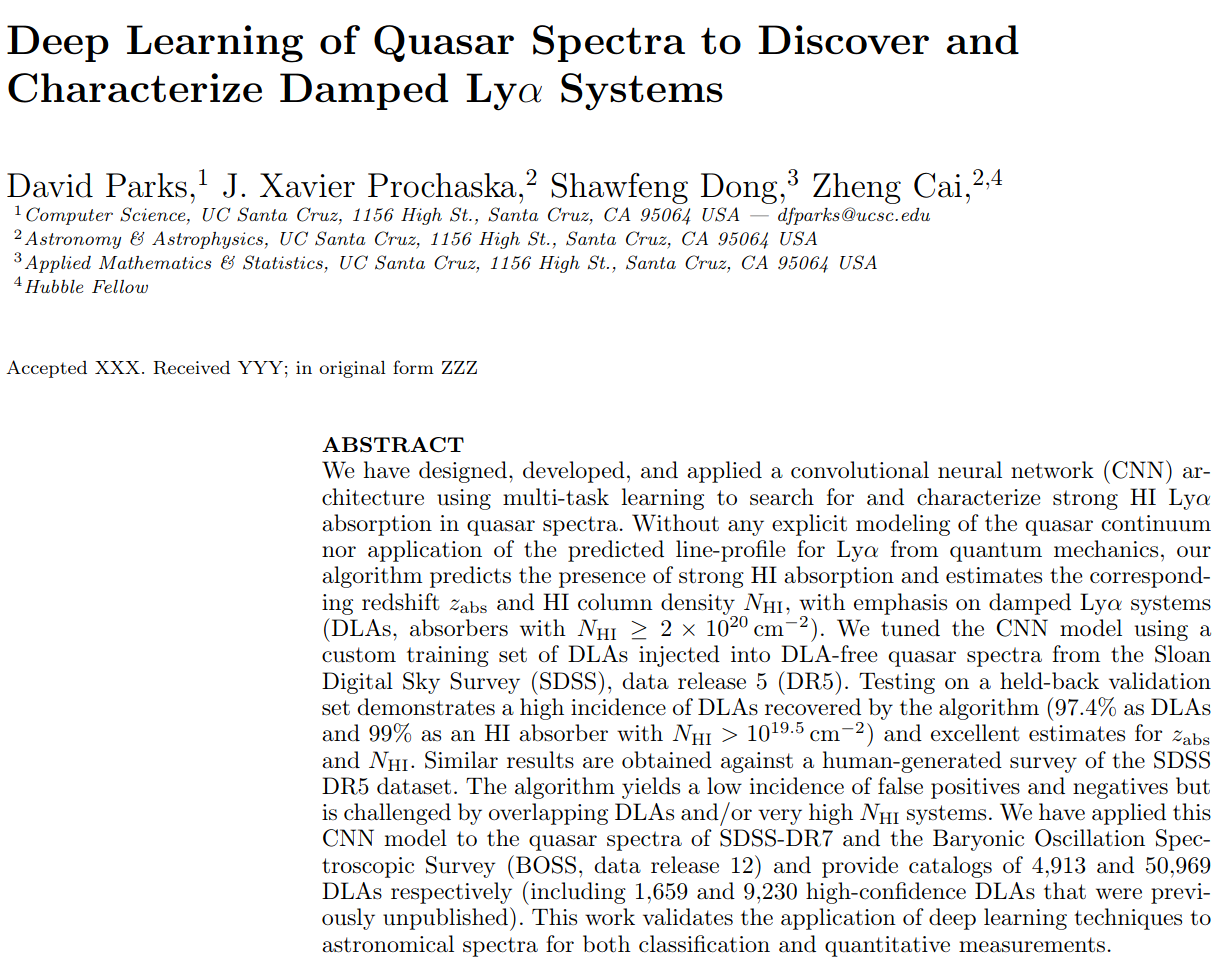
\includegraphics[height=7cm]{CNN-paper.png}
	
}


\frame{\frametitle{Training   DLA/noDLA models: 1D image recognition}
	\centering

	\uncover<1->{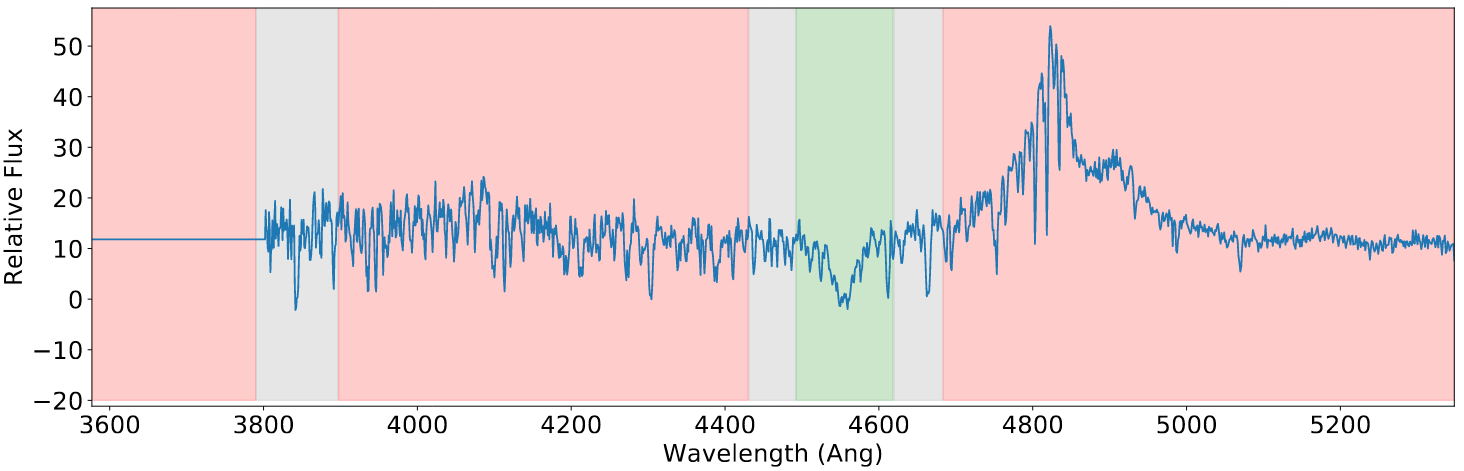
\includegraphics[height=3cm]{DLA-train}}
	\uncover<2->{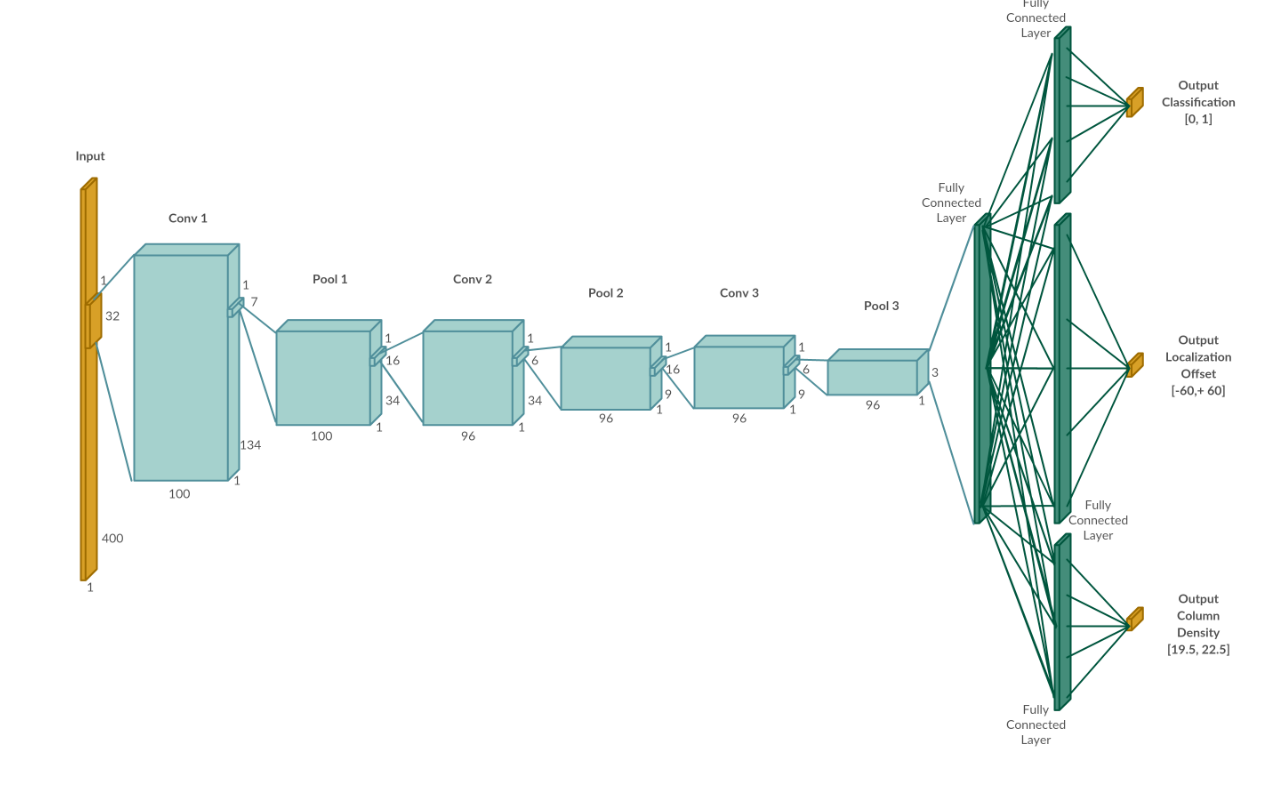
\includegraphics[height=5cm]{1d_DLA}}
	
}
%\subsection{Gaussian Processes}
%\frame{\frametitle{How Gaussian Processes works?}
%	\centering
%	%\includemovie{1cm}{1cm}{svm1.gif}	
%	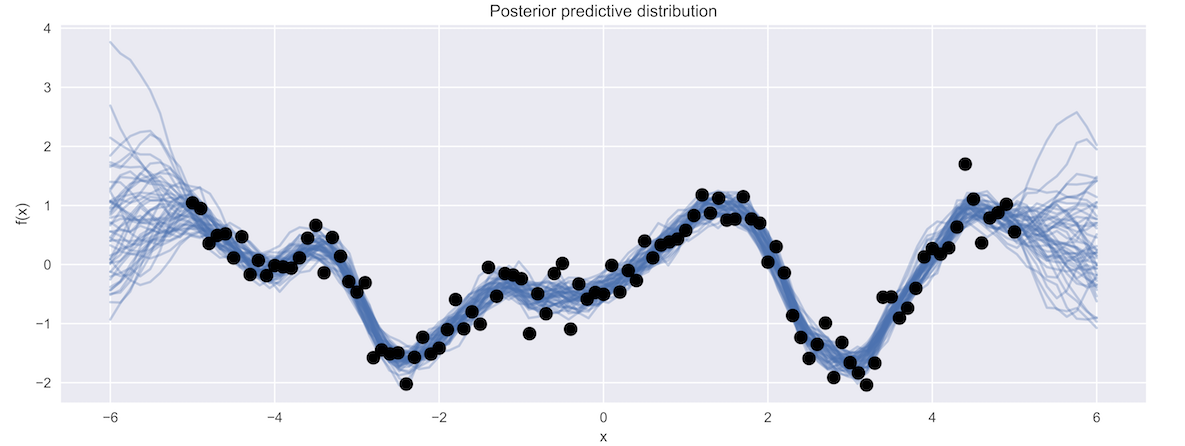
\includegraphics[width=\linewidth]{GP-works}
%	
%}
%
%\frame{\frametitle{Gaussian Processes and DLAs?}
%	\centering
%	%\includemovie{1cm}{1cm}{svm1.gif}	
%	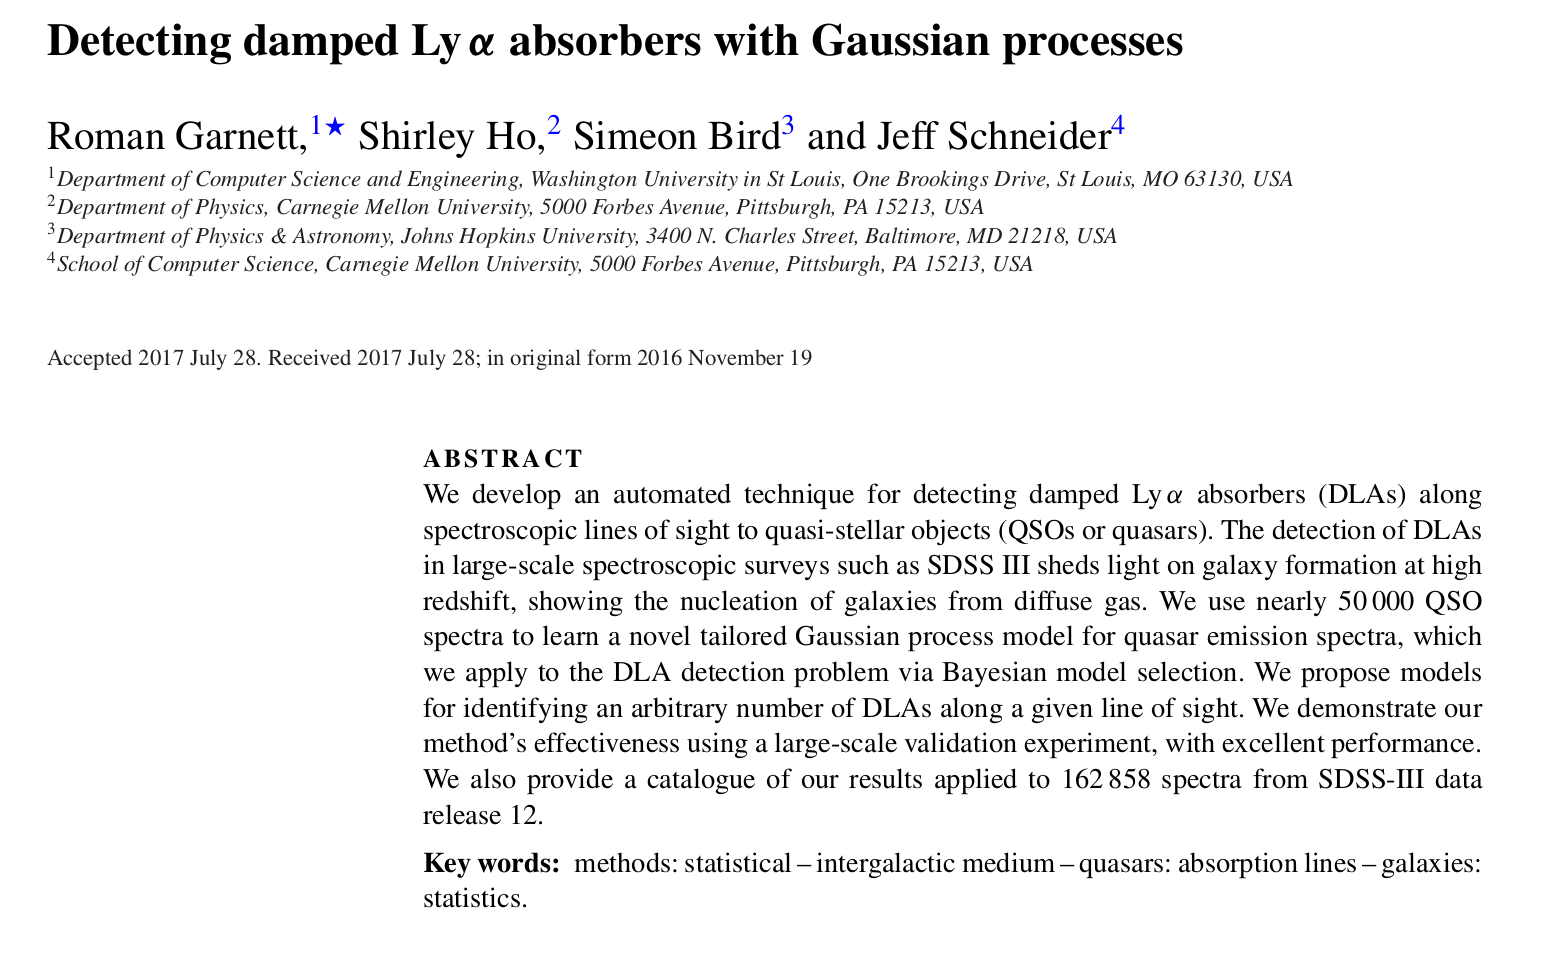
\includegraphics[width=\linewidth]{GP-paper}
%	
%}
%\frame{\frametitle{Posterior Probability: DLA$_-$} 
%	
%	\centering
%	%\includemovie{1cm}{1cm}{svm1.gif}	
%	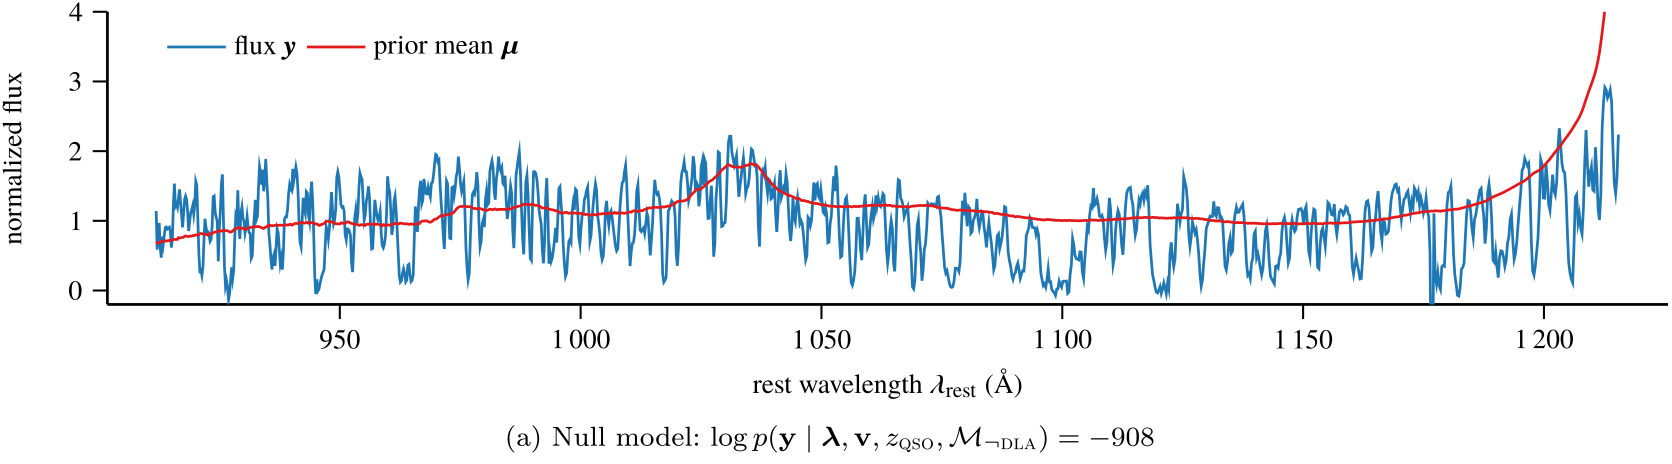
\includegraphics[width=\linewidth]{P-noDLA}
%	
%}
%\frame{\frametitle{Posterior Probability: DLA$_+$} 
%	
%	\centering
%	%\includemovie{1cm}{1cm}{svm1.gif}	
%	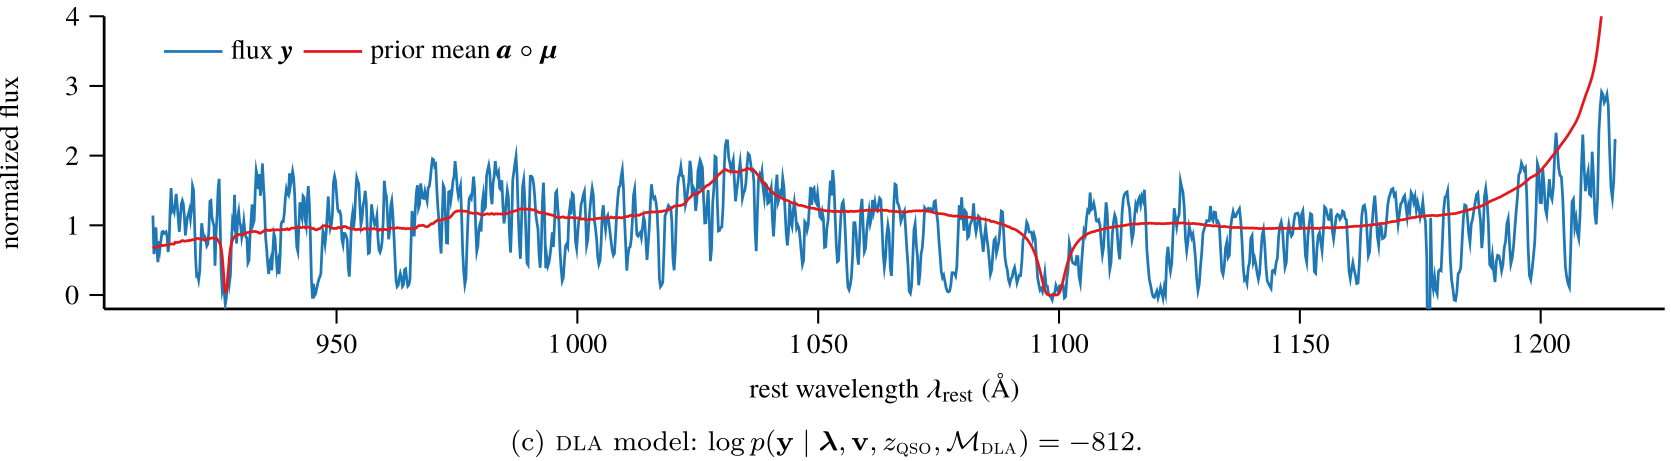
\includegraphics[width=\linewidth]{P-DLA}
%	
%}
%
%
%




%\frame{\frametitle{Stages of Supervised Learning} 
%\centering
%\includegraphics[width=\linewidth]{.jpg}
%}

%\frame{ \frametitle{Supervised Learning vs Traditional Model Fitting ?}
%
%\uncover<1->{\begin{bclogo}{Similarities}
%		\begin{itemize}
%			\uncover<2->{\item Both need a set of labeled measurements and a model }
%				
%		\end{itemize} 
%	\end{bclogo}}
%\uncover<3->{\begin{bclogo}{Differences}
%		\begin{itemize}
%				\uncover<4->{ \item SML: model is constructed based on input data}
%				\uncover<5->{\item SML: model can be very nonlinear/complex }
%				\uncover<6->{\item TMF: model is predefined and has limited adaptivity}
%				\uncover<7->{\item SML: designed for predicting unseen data}
%			\uncover<8->{\item TMF: infers  relationships between  features}
%		\end{itemize} 
%\end{bclogo}}	
}

\section{Unsupervised ML}
\subsection{Overview}
\frame {\frametitle{How unsupervised learning works?}
	\centering

%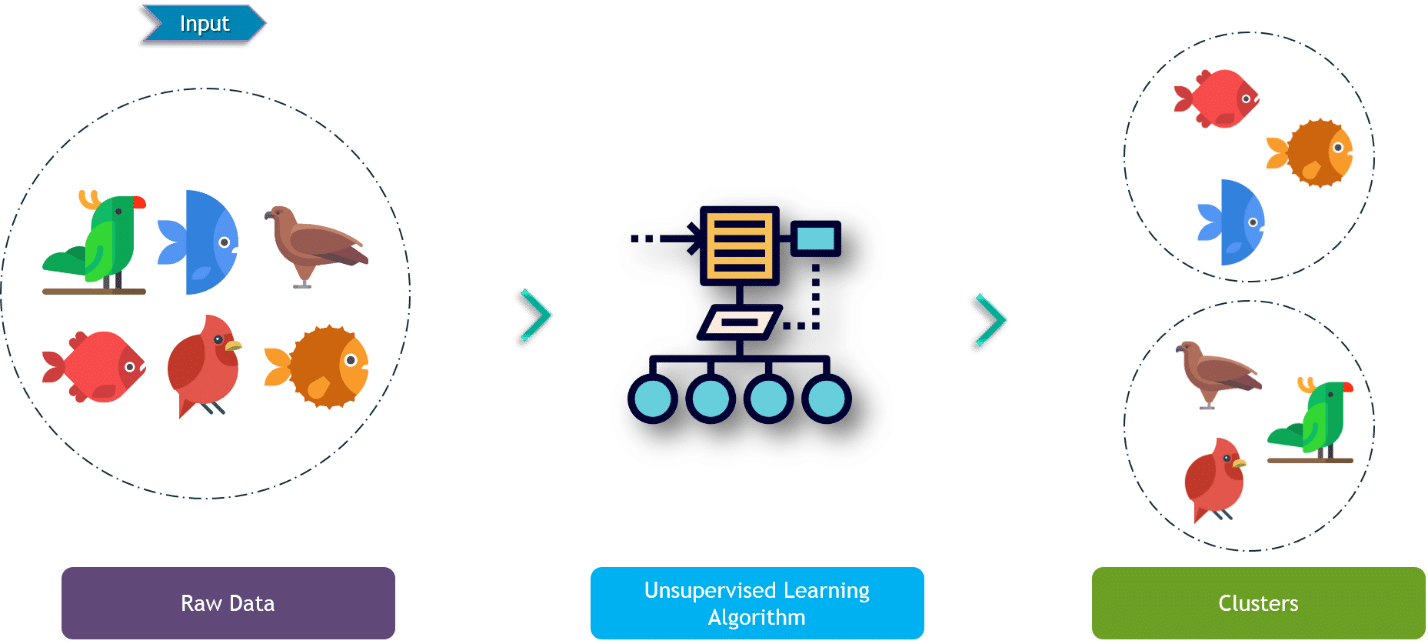
\includegraphics[width=0.7\linewidth, angle=90]{unsuper}
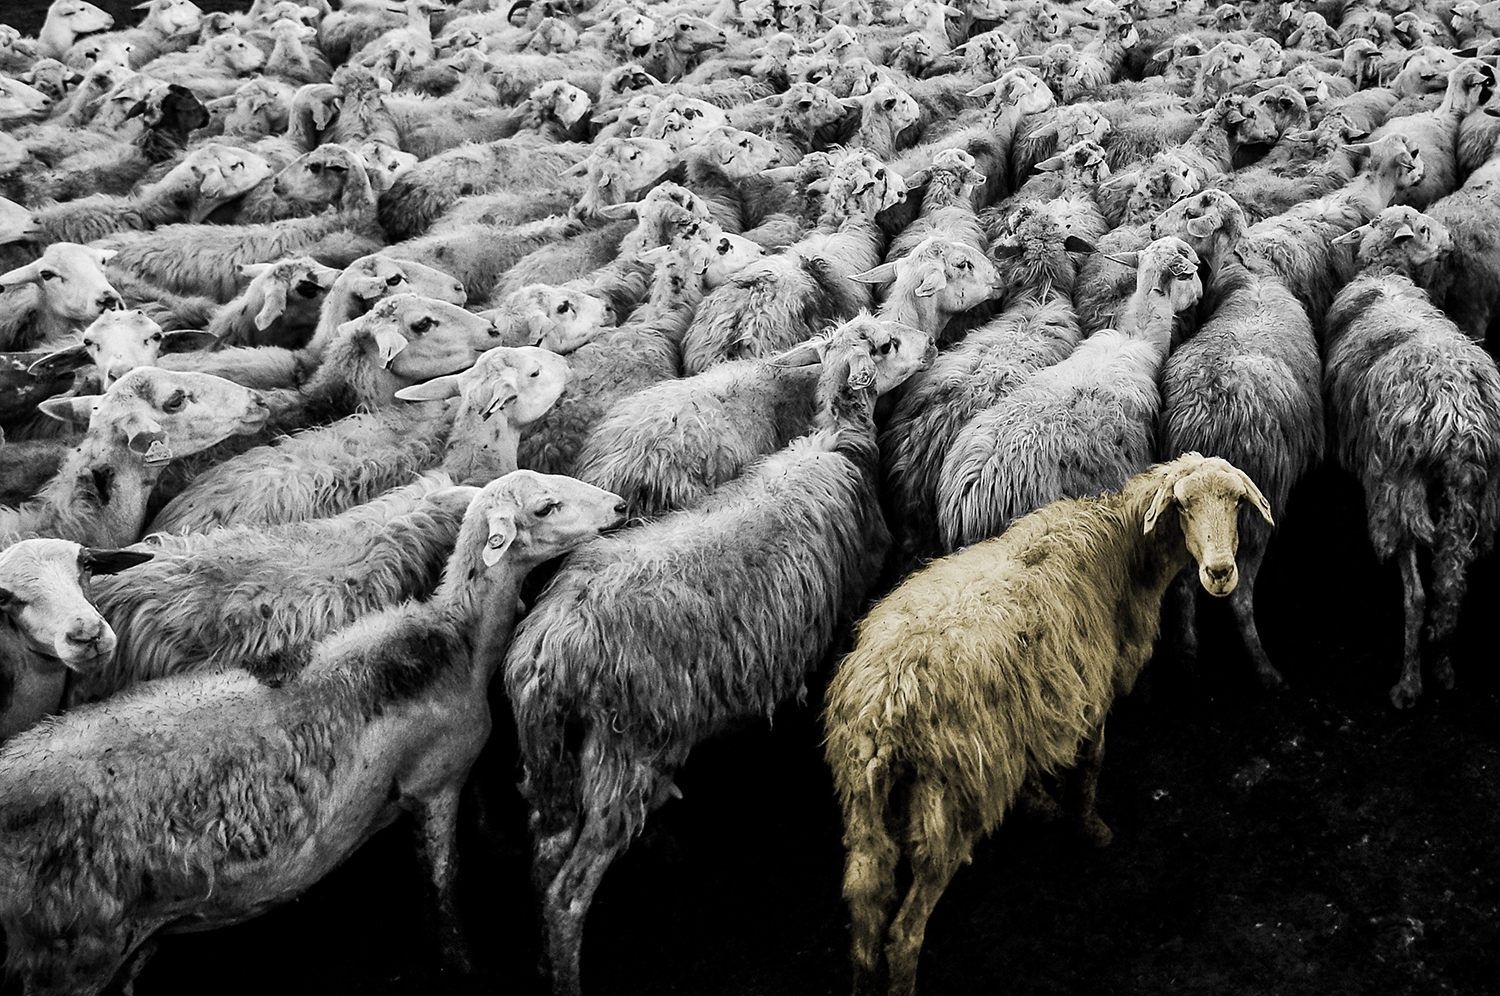
\includegraphics[width=0.3\linewidth, angle=10]{outlier-1}
	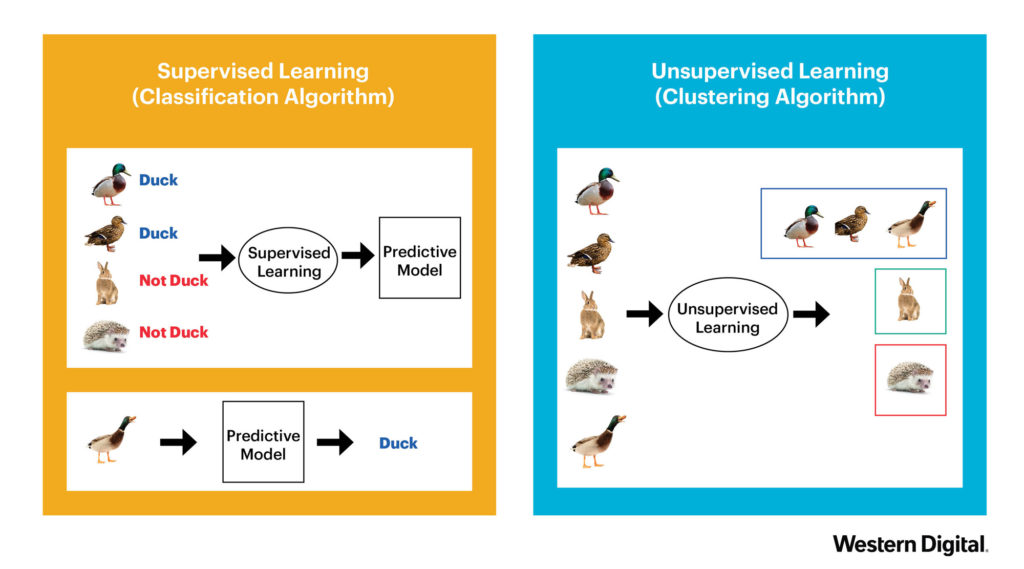
\includegraphics[width=0.7\linewidth]{super}}

\frame{\frametitle{Unsupervised Learning and knowledge discovery}
	\begin{itemize}
		\uncover<1->{\item Clustering: \\ \textcolor{red}{Distinguishing similar objects and patterns in the data-set}}
		\uncover<2->{\item Anomaly detection: \\ 
			\textcolor{red}{Recognizing odd objects which cannot be categorized and do not belong to any group  in the data-set}}
	\uncover<3->{\item Visualizationand dimentionality reduction: \\
			\textcolor{red}{Maping high dimensional data set to a  2D or 3D space}}
	\end{itemize}

%\uncover<4->{\begin{block}{}
%		\centering
%		\huge{DATA $\xrightarrow{ML}$ Knowledge} 
%		
% \end{block}}	
}

%\frame{ \frametitle{Unsupervised Learning Tasks}
%	\Large
%	\begin{itemize}
%		\uncover<1->{\item Clustering}
%		\uncover<2->{\item Anomaly detection }
%	\uncover<3->{\item Dimensionality Reduction (Visualization)}
%	\end{itemize}
%}
%\subsection{Kmeans Clustering}
%\frame{\frametitle{How KMeans clustering works?}
%	\centering
%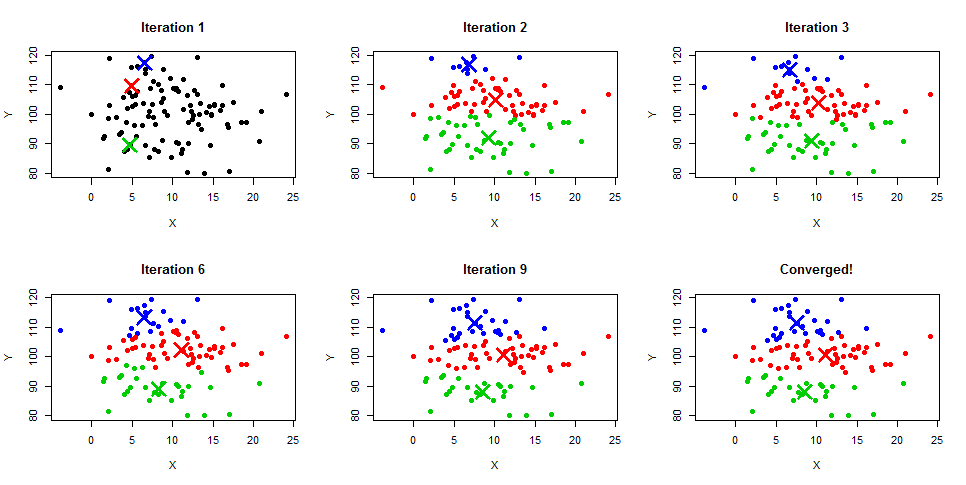
\includegraphics[width=\linewidth]{kmeans-works}
%}
%
%\frame{\frametitle{KMeans and Spectral Classification}
%	\centering
%	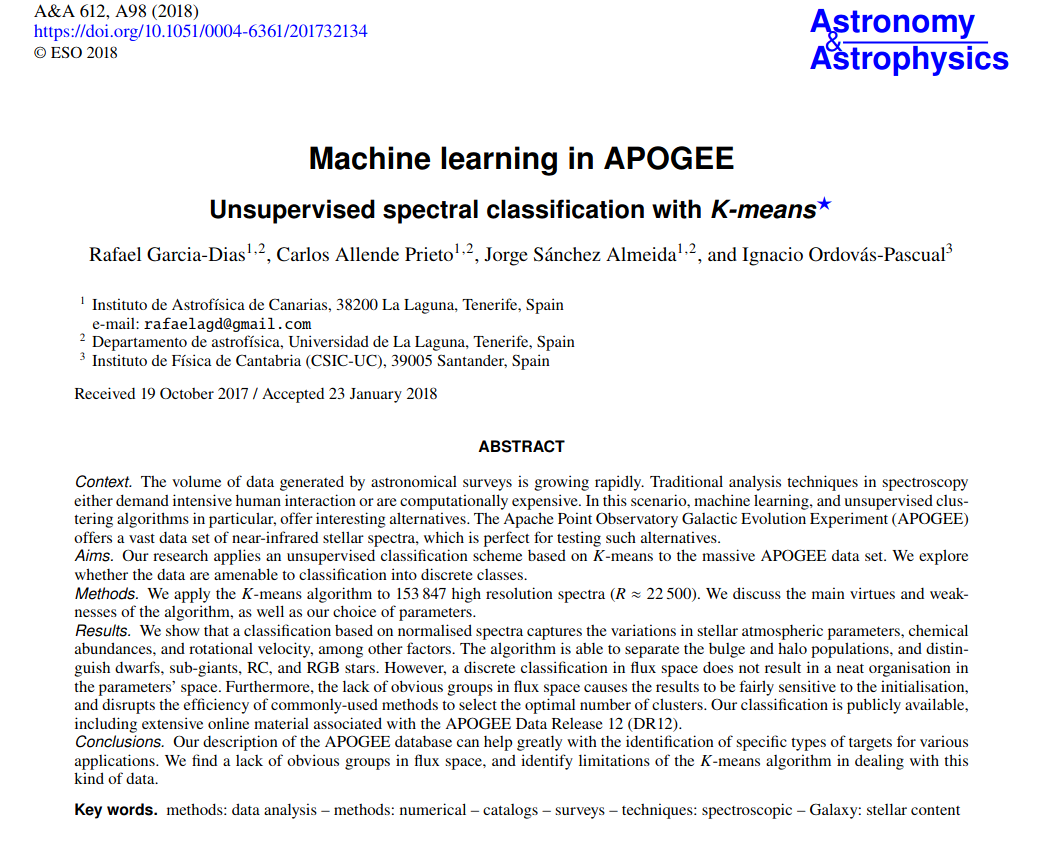
\includegraphics[width=\linewidth]{kmeans-paper}
%}
%
%\frame{\frametitle{KMeans and Spectral Classification}
%	\centering
%
%	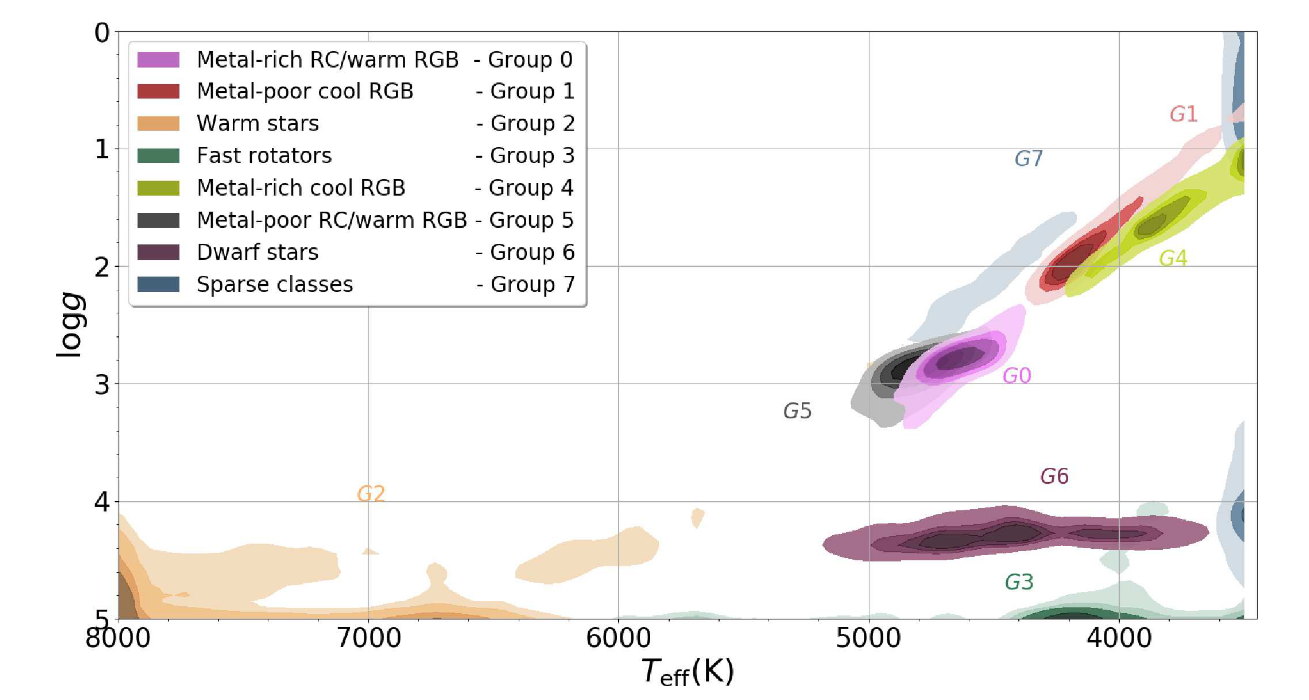
\includegraphics[width=\linewidth]{kmans-classes-T-G}
%	}


\subsection{Agglomerative clustering}
\frame{\frametitle{How Agglomerative clustering works?}
	\centering
	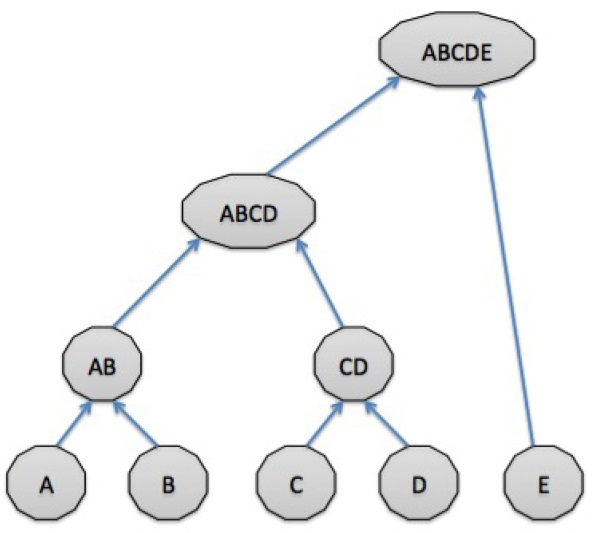
\includegraphics[height=6cm]{Agg-works}
}
\frame{\frametitle{Linkage methods in Agglomerative clustering?}
	\centering
	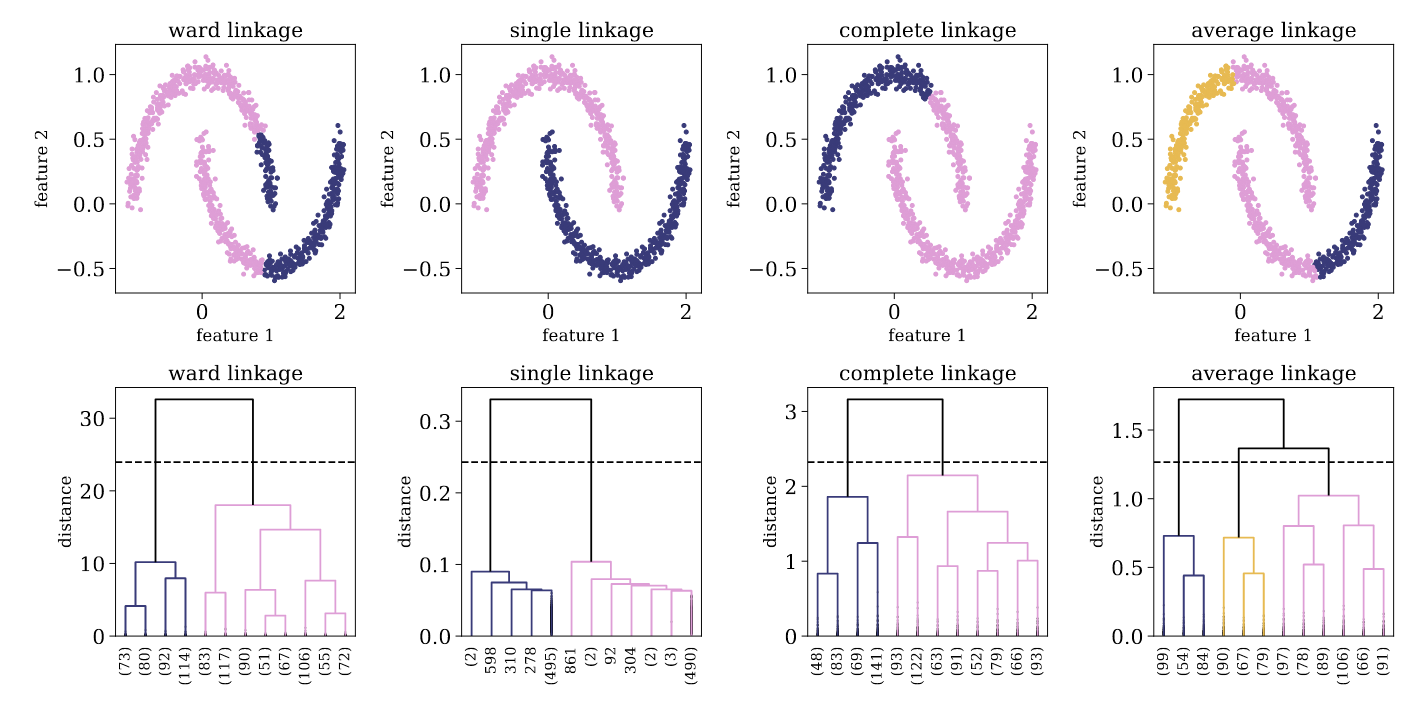
\includegraphics[width=\linewidth]{Agg-Lk}
}
\frame{\frametitle{Agglomerative clustering finds weird quasars?}
	\centering

	\uncover<1->{\includegraphics[width=0.7\linewidth]{3d-agg-4-cl-link-average}}
    \uncover<2->{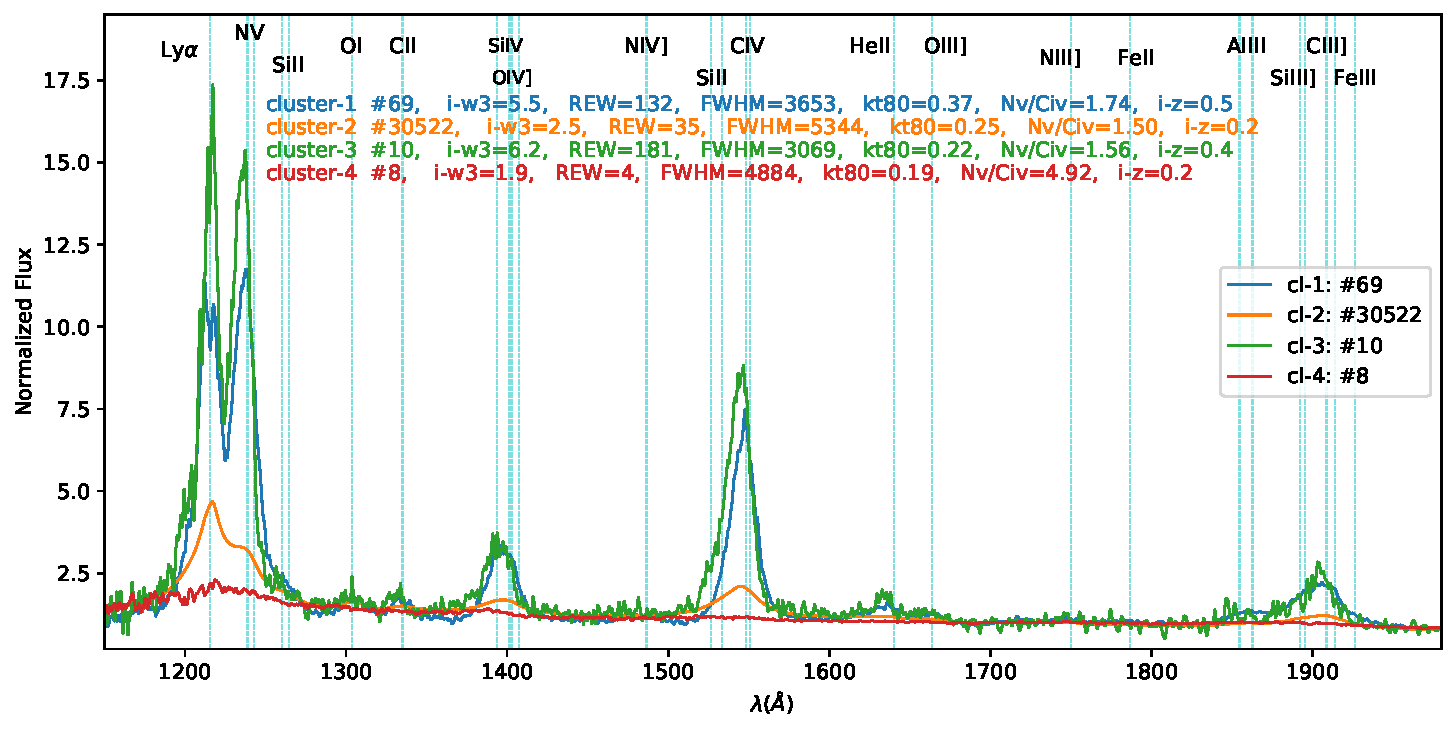
\includegraphics[width=0.7\linewidth]{3d-agg-link-average-nCl-4-med-spec-1150-1980}}
}

\subsection{LOF }
\frame{ \frametitle{ Local Outlier Factor finds outliers}
	\centering
	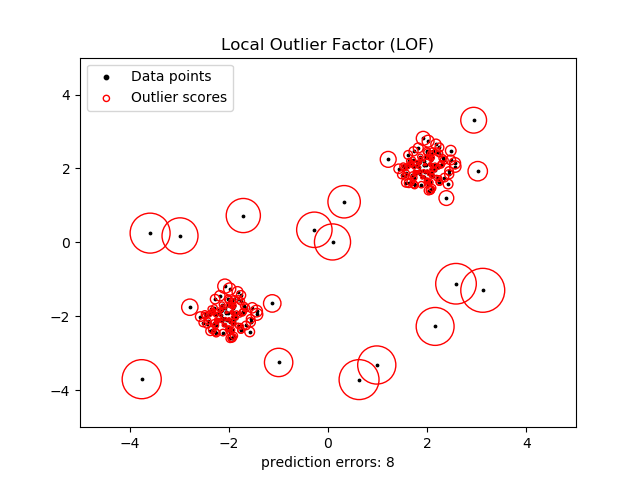
\includegraphics[height=6cm]{LOF-works}
}
\subsection{PCA}
\frame{\frametitle{Dimensionality Reduction with Principal Component Analysis}
\centering
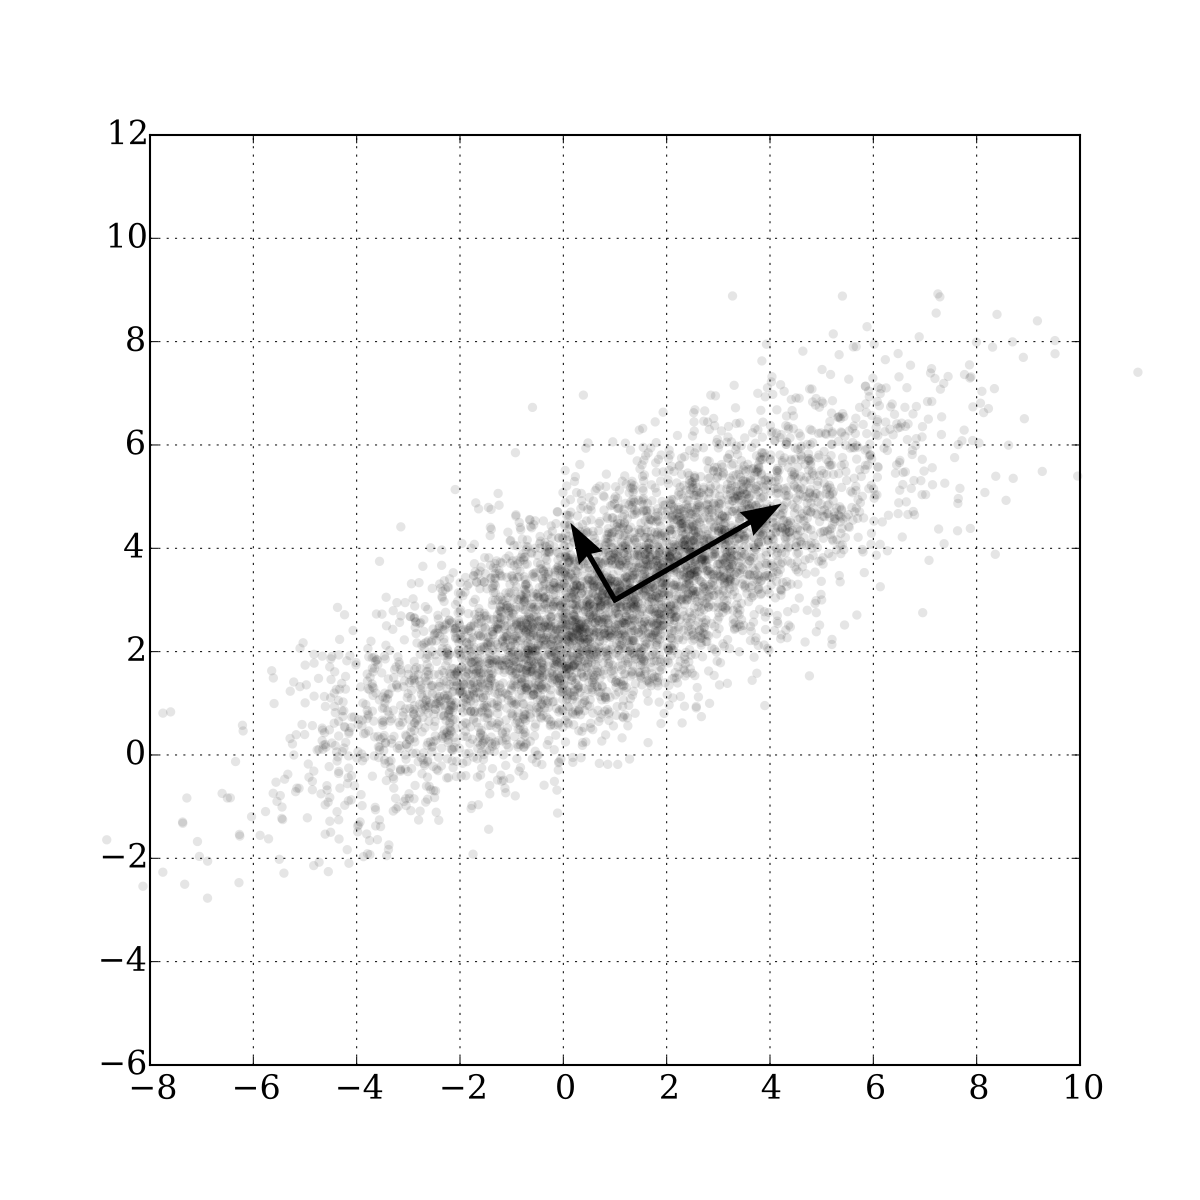
\includegraphics[height=7cm]{PCA-works}
}
\subsection{tSNE}
\frame{\frametitle{Visualization  with t-Distributed Stochastic  Neighbor Embedding}
\centering
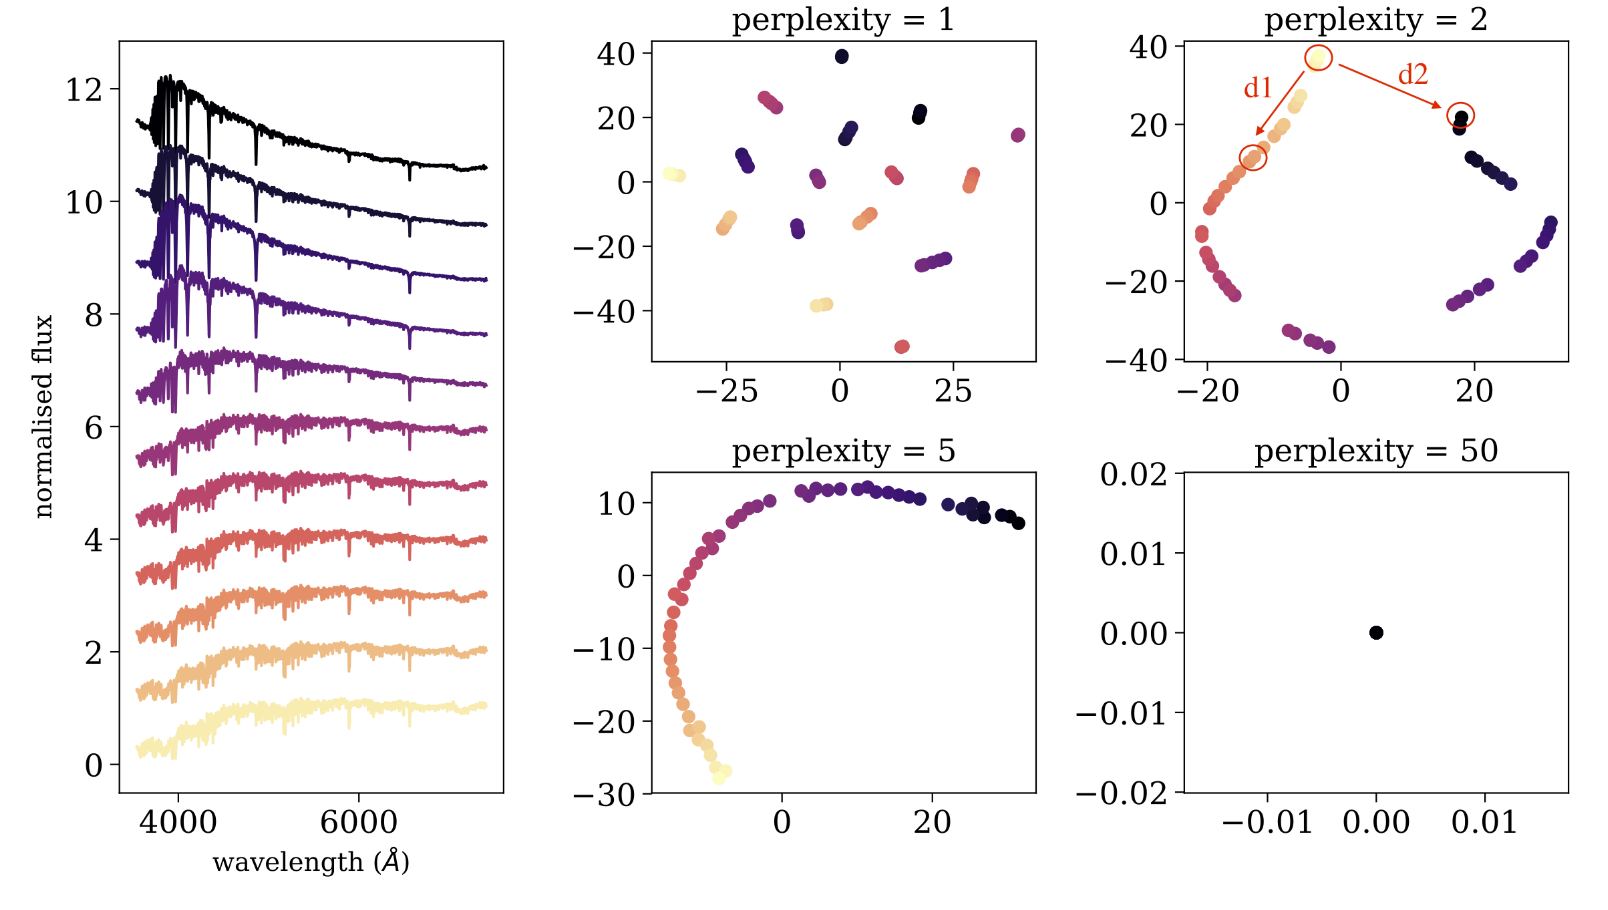
\includegraphics[width=\linewidth]{tSNE.png}
}
%\subsection{Neural network}\frame{text}
%}
%
%\section{ML and SKA}
%\frame{}
\section{ML limitations
}{ 
	\frame{\frametitle{Limitation of ML in astronomy}
		\begin{itemize}
			\uncover<1->{\item Lack of Pre-procession and normalization can end up with misleading/wrong results }
			\uncover<2->{\item ML algorithms are mostly designed for industry not science. }
			\uncover<3->{\item Training on a biased sample is very dangerous }
			\uncover<4->{\item ML is not plug and play}
			\uncover<5->{\item There are a variety of methods for each task}
			\uncover<6->{\item Some algorithms scarify interpretablity for functionality
			  }
		\end{itemize}
	
}

%\section{Summary}
\section{References}{
%}
\frame{\frametitle{References}\begin{enumerate}
		\small
		\item \textbf{ML, General:} Baron, Dalya. \textcolor{red}{"Machine learning in astronomy: A practical overview."} arXiv preprint arXiv:1904.07248 (2019).
	
		
		\item \textbf{Big Data:} Zhang, Yanxia, and Yongheng Zhao. \textcolor{red}{"Astronomy in the big data era."} Data Science Journal 14 (2015).
		
		\item \textbf{SVM:} Ksoll, Victor F., et al. \textcolor{red}{"Hubble Tarantula Treasury Project–VI. Identification of pre-main-sequence stars using machine-learning techniques."} Monthly Notices of the Royal Astronomical Society 479.2 (2018): 2389-2414.
		
		\item \textbf{Decision Tree:} Vasconcellos, E. C., et al. \textcolor{red}{"Decision tree classifiers for star/galaxy separation."} The Astronomical Journal 141.6 (2011): 189.
		\item \textbf{Neural Network:} Parks, David, et al. \textcolor{red}{"Deep learning of quasar spectra to discover and characterize damped Lyα systems."} Monthly Notices of the Royal Astronomical Society 476.1 (2018): 1151-1168.
		
		
		
		\item \textbf{Agglomerative clustering:} R. Monadi, F. Hamann, S. Bird, \textcolor{red}{Precise Selection of Extremely Red Quasars}, (in preparation)
		
		
		
		
		
	
	\end{enumerate}}
}
\section{}
\frame{
\huge
\centering

\includegraphics[width=0.8\linewidth]{thanku-2}
}
\end{document}